%&pdflatex
\documentclass[12pt]{article}
\usepackage{algorithmicx}
\usepackage[ruled]{algorithm}
\usepackage{algpseudocode}
\usepackage{algpascal}
\usepackage{algc}
\usepackage{url,enumerate, amssymb, anysize, booktabs, amsfonts}
\usepackage[colorlinks = true,
linkcolor = blue,
urlcolor  = blue,
citecolor = green,
anchorcolor = blue]{hyperref}
\usepackage{setspace,listings}
\usepackage[dvipdfmx]{graphicx}
\usepackage{amsmath}
\usepackage{psfrag}
\usepackage[font=small,labelfont=bf]{caption}
\usepackage{enumerate}
\usepackage{natbib}
\usepackage{url} % not crucial - just used below for the URL 

% NOTE: To produce blinded version, replace "0" with "1" below.
\newcommand{\blind}{1}

% DON'T change margins - should be 1 inch all around.
\addtolength{\oddsidemargin}{-.5in}%
\addtolength{\evensidemargin}{-.5in}%
\addtolength{\textwidth}{1in}%
\addtolength{\textheight}{-.3in}%
\addtolength{\topmargin}{-.8in}%
\usepackage{color,amssymb}
\usepackage{fancyhdr, mathtools}
\usepackage{dcolumn}
\usepackage{indentfirst, verbatim}
%\newcounter{equationset, sectsty, breqn}
\usepackage{setspace,float,lscape,amsmath,color}
\usepackage{color,amssymb}
\usepackage{fancyhdr, mathtools, amsthm}
\theoremstyle{definition}
\newtheorem{definition}{Definition}[section]
\newtheorem{theorem}{Theorem}[section]
\newtheorem{corollary}{Corollary}[theorem]
\newtheorem{lemma}[theorem]{Lemma}
\newtheorem{remark}{Remark}


\newcommand{\Linefor}[2]{%
	\State \algorithmicfor\ {#1}\ \algorithmicdo\ {#2} \algorithmicend\ \algorithmicfor%
}
\newcommand{\Lineif}[2]{%
	\State \algorithmicif\ {#1}\ \algorithmicdo\ {#2} \algorithmicend\ \algorithmicif%
}


\renewcommand{\algorithmicrequire}{\textbf{Input:}}
\renewcommand{\algorithmicensure}{\textbf{Output:}}

%\usepackage{algorithmicx}

%\algdisablelines

\begin{document}
	
	%\bibliographystyle{natbib}
	
	\def\spacingset#1{\renewcommand{\baselinestretch}%
		{#1}\small\normalsize} \spacingset{1}
	
	
	%%%%%%%%%%%%%%%%%%%%%%%%%%%%%%%%%%%%%%%%%%%%%%%%%%%%%%%%%%%%%%%%%%%%%%%%%%%%%%
	
	\if1\blind
	{
		\title{\bf Testing independence between networks and nodal attributes via multiscale metrics}
		\author{Youjin Lee\thanks{
				The authors gratefully acknowledge \textit{please remember to list all relevant funding sources in the unblinded version}}\hspace{.2cm}\\
			Department of Biostatistics, Johns Hopkins School of Public Health\\
			and \\
			Author 2 \\
			Department of ZZZ, University of WWW}
		\maketitle
	} \fi
	
	\if0\blind
	{
		\bigskip
		\bigskip
		\bigskip
		\begin{center}
			{\LARGE\bf Testing independence between networks and nodal attributes via multiscale metrics}
		\end{center}
		\medskip
	} \fi
	
	
\sloppy
\bigskip
\begin{abstract}
	%The text of your abstract. 200 or fewer words.
		Network dependence, which refers to the dependence between network topology and its nodal attributes, often exhibits nonlinear patterns. Unfortunately, without knowledge on metrics defined over network, no statistic has been proposed to test network dependence further beyond globally linear dependence. This paper introduces a multiscale dependence test statistic called Multiscale Network Test (\texttt{MNT}), which borrows the idea from diffusion maps and Multiscale Generalized Correlation (\texttt{MGC}). Our method can be applied to any exchangeable graph under some mild conditions, without further model assumption nor estimation. We prove the consistency of test statistic and demonstrate superior performance than any other model-based, global test statistics. Simulation in a variety of networks shows higher power of test, especially in stochastic block model under nonlinear dependency. The application to dMRI networks will be followed. 
\end{abstract}
	
	\noindent%
	{\it Keywords:} distance correlation, multiscale generalized correlation, diffusion maps, exchangeable graph, stochastic block model 
	\vfill
	
	\newpage
	\spacingset{1.45} % DON'T change the spacing!
	\section{Introduction}
	\label{sec:intro}

Network, a collection of nodes and edges between them, has been a celebrated area of study over a field of sociology \citep{pinquart2000influences, ellison2007benefits}, information theory \citep{gross2005information}, biology \citep{barabasi2004network, pujol2010unveiling}, statistics \citep{raftery2012fast, palla2012infinite}, economics \citep{banerjee2013diffusion}, etc. The correlation between network relationship between nodes and their attribute values is a common interest in network analysis. According to an assumption on how they are related each other, there has been lots of efforts to manifest a network as a function of nodal attributes \citep{wasserman1996logit, howard2016understanding} or model an outcome of nodal attribute variables through their underlying network structures \citep{christakis2007spread, christakis2008collective}. However, it is very obscure to determine which one should be put as a dependent variable or even whether networks are truly related to nodal attributes and how they are, if any. Moreover, a fundamental difficulty comes from the empirical fact that network often does not have a natural structure. Thus it is not easy to intuitively come up with how to represent network as a node-specific random variable. \cite{fosdick2015testing} overcomes this issue by estimating network factors which are believed to embody each node's locations in network space. These factors are in the end used to test independence between network topology and nodal attributes by implementing standard statistical testing method. Through allowing us to choose the dimension of latent factors, they make up the constraints of parametric modeling. However their statistical modeling on networks still rely on the assumption that all the nodes in network would follow the same pattern of dependence -- subject to additive and multiplicative effect. This might not be true for always. In this paper we develop a nonparametric test statistic which is also sensitive to nonlinear and local dependence pattern.  

\begin{figure}[h]
	\centering
	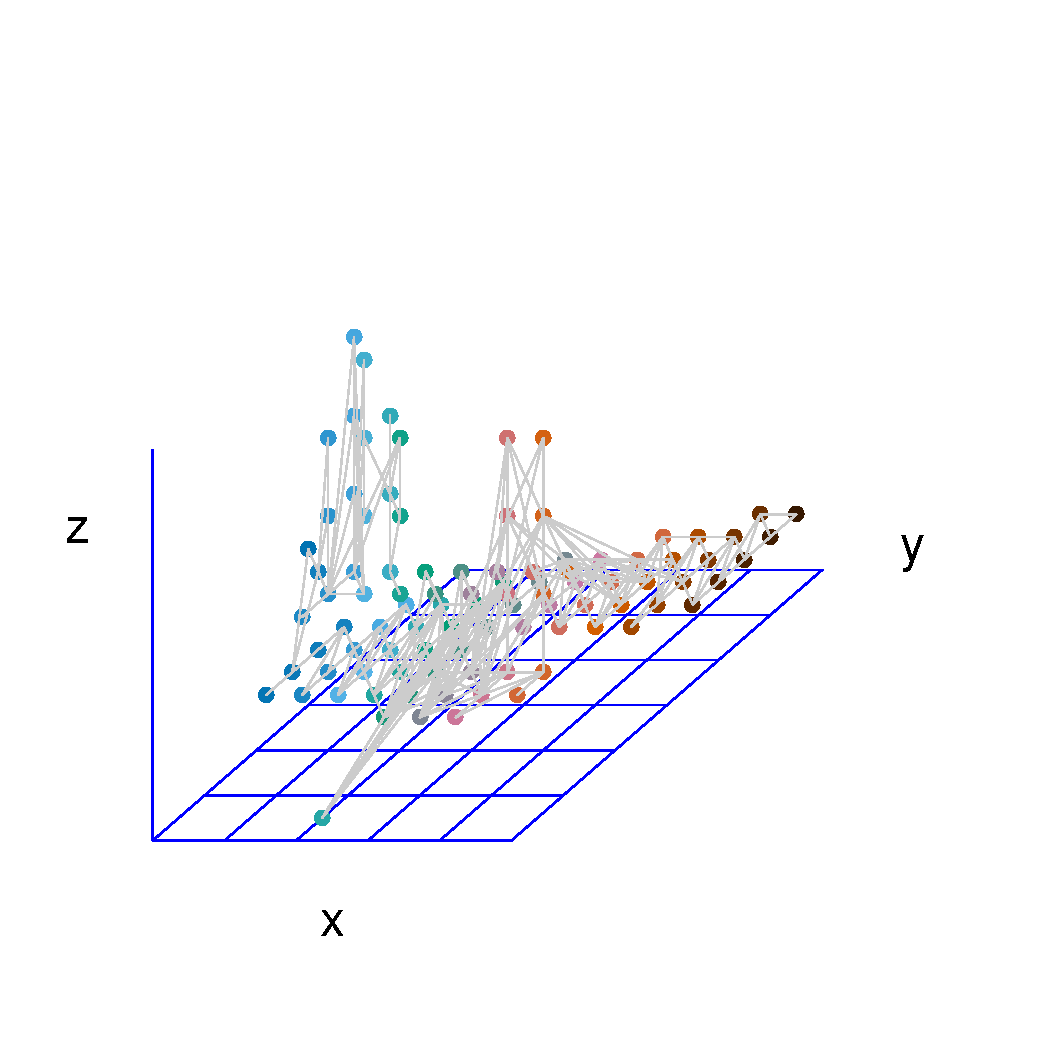
\includegraphics[width=4in]{../Figure/intro.pdf}	
	\caption{Physical location of one component of human brain network and its tracts that connect one vertex to another.}
	\label{fig:intro}
\end{figure}

Throughout this paper, assume that we are given an unweighted and undirected, connected network, equivalently a graph $\mathbf{G}$ without self-loop, comprised of $n$ nodes for a fixed $n \in \mathbb{N}$. Even though we assume that $\mathbf{G}$ is undirected and unweighted, we are able to extend all of the theory here to directed and even weighted network. An adjacency matrix of a given network, denoted by $\mathbf{A} = \{A_{ij} : i,j= 1,..,n \}$, is often introduced to formalize the relational data of network, where $A_{ij} = 1$ if node $i$ and node $j$ are adjacent each other and zero otherwise. Let us introduce a $m$-variate ($m \in \mathbb{N}$) variable for nodal attributes $\mathbf{X}  \in \mathbb{R}^{m}$ which we are interested in. Investigating correlation between $\mathbf{G}$ and $\mathbf{X}$, i.e. testing whether their distributions are independent or not is a key focus in our study. An observed network $\mathbf{G}$ can represent social network within a school and $\mathbf{X}$ is students' grades or heights, for example; or $\mathbf{G}$ can be a neuronal network in human brain and $\mathbf{X}$ is a few factors of personality. For example, Figure~\ref{fig:intro} exemplifies one connected network from human brain where dots denote nodes and tracts connected them represent edges. Location over network space, i.e. whether or how much a pair of nodes are closer than the others, is different from actual spatial location, which can be measured by Euclidean distance over three-dimensional $xyz$ space. As correlation between spatial location of subjects and its attributes has been studied, we are going to explore correlation of subjects' attributes to their network location. 
	
The main contribution of this study is to develop multiscale test statistics for network independence which are robust to both nonlinearity and high dimensionality without modeling nor estimating networks. Having multiscale statistics is not avoidable because we regard location of or distance between nodes over network as a dynamic process. We then choose the optimal scale where distance in network space and distance in attributes maximize their correlation. To parse into this time-dependent distances, we construct a coordinate over network space and test independence to attributes $\mathbf{X}$ at each time in the process. In the next methodology section~\ref{sec:method}, we are going to introduce a test statistic using multiscale distance metrics which inherit desirable properties. In section~\ref{sec:sim}, numerical results demonstrate the best performance of our method compared to the existing under various circumstances. Real data example in section~\ref{sec:real} show one of the applications among many.  
	
%%%%%%%%%%%%%%%%%%%%%%%%%%%%%%%%%%%%%%%%%%
\bigskip
\section{Methodology}
\label{sec:method}

\subsection{Multiscale Generalized Correlation}

Relationship between network and nodal attributes often exhibits local or nonlinear properties. For example, it is likely that attributes of some subjects may be affected by their network relationship but those of the others are not; or that attributes are correlated on network only when network relationships are too week or too strong. Moreover, we could expect that dimension of network spectrum increases as the number of nodes increases. Unfortunately, widely used correlation measures often fail to capture nonlinear associations especially embedded in high-dimensional data set. \cite{szekely2007measuring} extended pairwise constructed generalized correlation coefficient and developed a novel statistic called distance correlation (\texttt{dCorr}) as a measure for all types of dependence between two random vectors in any dimension.

Let us first start from a general setting that we are given $n \in \mathbb{N}$ pairs of \textit{i.i.d} random samples $\big(  \mathbf{X}, \mathbf{Y}  \big)  = \{ (\mathbf{x}_{i}, \mathbf{y}_{i}) : \mathbf{x}_{i} \in \mathbb{R}^{q}, \mathbf{y}_{i} \in \mathbb{R}^{m}, i = 1,...,n \}$. Define $C_{ij} = \parallel \mathbf{x}_{i} - \mathbf{x}_{j} \parallel$ and $D_{ij} = \parallel \mathbf{y}_{i} - \mathbf{y}_{j} \parallel$ for $i,j=1,2, \ldots ,n$, where $\parallel \cdot \parallel$ denotes Euclidean distance of any vectors.   
Distance correlation (\texttt{dCorr}) is defined via distance covariance (\texttt{dCov}) $\mathcal{V}^2_{n}$ of $\mathbf{X}$ and $\mathbf{Y}$, which is the following: 
\begin{equation}	 
\mathcal{V}^2_{n}(\mathbf{X}, \mathbf{Y}) = \frac{1}{n^2} \sum\limits_{i,j=1}^{n} \tilde{C}_{ij} \tilde{D}_{ij},
\end{equation}
where $\tilde{C}$ and $\tilde{D}$ is a doubly-centered $C$ and $D$ respectively, by its column mean and row mean. Distance correlation $\mathcal{R}^{2}_{n}(\mathbf{X}, \mathbf{Y})$ is a standardized \texttt{dCov} scaled by $\mathcal{V}^2_{n}(\mathbf{X}, \mathbf{X})$ and $\mathcal{V}^2_{n}(\mathbf{Y}, \mathbf{Y}).$

\begin{figure}[H]
	\centering
	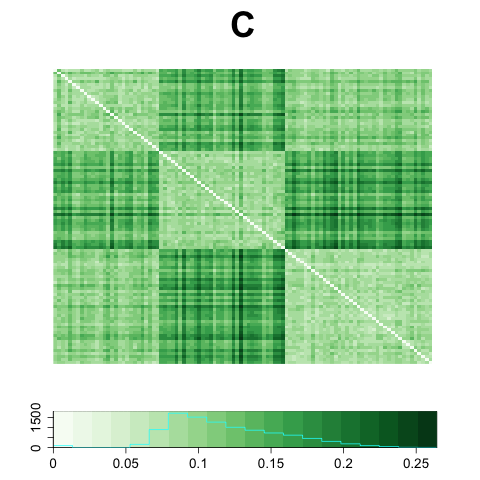
\includegraphics[width=1.5in]{../Figure/C.png}
	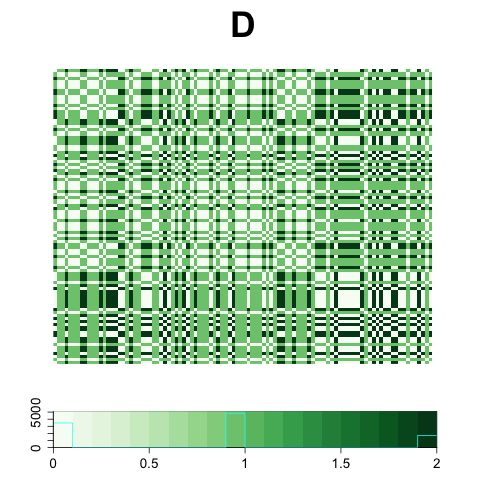
\includegraphics[width=1.5in]{../Figure/D.png}
	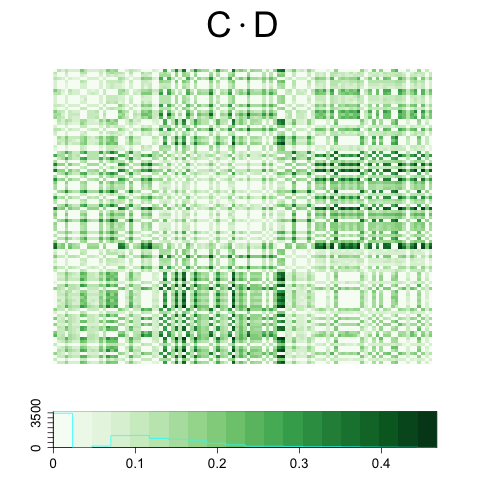
\includegraphics[width=1.5in]{../Figure/CD.png}
		
	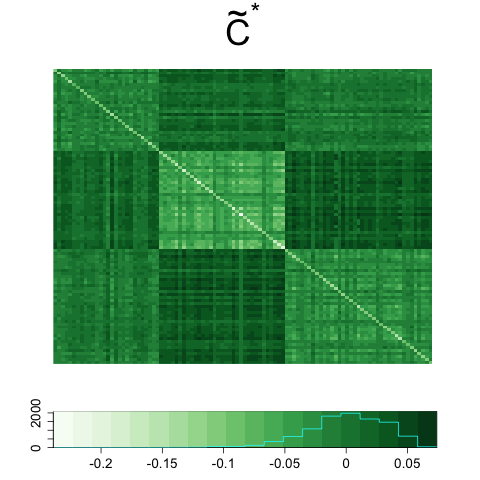
\includegraphics[width=1.5in]{../Figure/tildeCtrunc.png}
	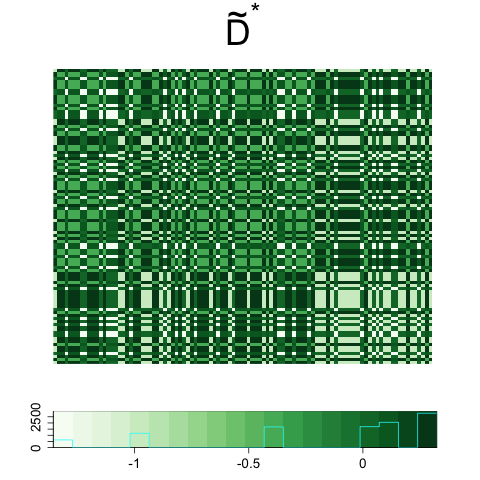
\includegraphics[width=1.5in]{../Figure/tildeDtrunc.png}
	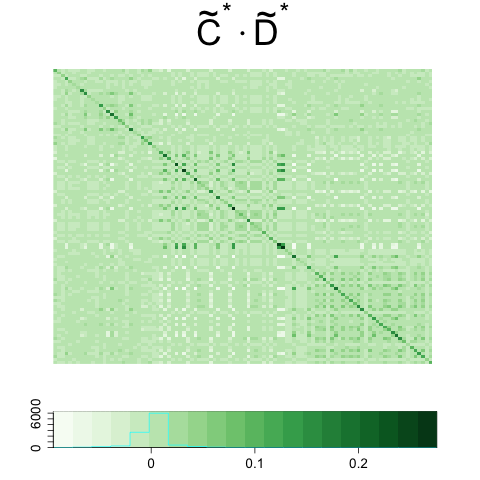
\includegraphics[width=1.5in]{../Figure/tildeCDtrunc.png}
	\caption{(a) Top : Euclidean distance of diffusion maps at time $t=3$, $C$; Euclidean distance of $X$, $D$; element-wise product of $C$ and $D$. (b) Bottom : truncated double-centered  $\tilde{C}$ by $k^{*}$th nearest neighbor in $C$; truncated double-centered $\tilde{D}$ by $l^{*}$th nearest neighbor in $D$; element-wise product of two truncated matrices $\tilde{C}^{*}$ and $\tilde{D}^{*}$. }
	\label{fig:MGCmatrices}
\end{figure}	

\begin{equation}	 
\mathcal{R}_{n}^{2} (\mathbf{X}, \mathbf{Y}) = \frac{\mathcal{V}^2_{n} (\mathbf{X}, \mathbf{Y}) }{\sqrt{\mathcal{V}^2_{n} (\mathbf{X}, \mathbf{X}) \mathcal{V}^2_{n} (\mathbf{Y}, \mathbf{Y}) } }
\end{equation}
In addition, a modified distance covariance (\texttt{mCov}) $\mathcal{V}^*_{n}$ and a modified distance correlation (\texttt{mCorr}) $\mathcal{R}^{*}_{n}$ for testing high dimensional random vectors were also proposed in \cite{szekely2013distance}.   
However, \texttt{dCorr} nor even \texttt{MCorr} still perform not very well in the existence of various nonlinear dependency and under existence of outliers [Cencheng]. Out of this concern, Cencheng at al (2016) proposed Multiscale Generalized Correlation (\texttt{MGC}) by adding local scale in a sense of nearest neighbors on correlation coefficients. Multiscale version of distance covariance $\{ { {\mathcal{V}^{*}}^2_{n} }   \}_{kl}$ is defined as following : 
\begin{equation}
\label{eq:MGC}
\begin{split}
{\mathcal{V}^{*}}^2_{n} (\mathbf{X}, \mathbf{Y})_{kl}  & = \frac{1}{n^2} \sum\limits_{i,j=1}^{n} \tilde{C}_{ij} \tilde{D}_{ij} I \big( r(C_{ij}) \leq k \big) I \big( r(D_{ij}) \leq l  \big) \\  
& = : \frac{1}{n^2} \sum\limits_{i,j=1}^{n} \tilde{C}^{*}_{ij} \tilde{D}^{*}_{ij},
\quad k,l=1,2,..., n ,
\end{split}
\end{equation}
where $r(C_{ij})$ ($r(D_{ij})$) denotes a rank $\mathbf{x}_{i}$ ($\mathbf{y}_{i}$) relative to $\mathbf{x}_{j}$ ($\mathbf{y}_{j}$). It basically truncates each pairwise element of distance covariance with respect to rank in terms of (Euclidean) distance. Note that if $k=l=n$, $\mathcal{V}^2_{n}$ and ${\mathcal{V}^{*}}^2_{n}$ are equivalent. You can see panels to illustrate both Euclidean distance matrices and truncated, double-centered Euclidean distance matrices in Figure~\ref{fig:MGCmatrices}. Simply speaking, given an appropriate distance matrix for $\{  \mathbf{x}_{i}  : i = 1,2, \ldots, n \}$ and $\{ \mathbf{y}_{i} : i=1,2,\ldots, n \}$ each, we take an double centering and truncate them by column ranking up to $k$ and $l$ in order to obtain $\tilde{C}^{*}$ or $\tilde{D}^{*}$ respectively. Since we call all family of $\{  {\mathcal{R}^{*}}^2_{n} \}_{k,l = 1,2,...,n}$ as \texttt{MGC}, \texttt{MGC} is more generalized version of \texttt{dCorr}. How to choose the optimal neighborhood scale of $(k,l)$, say $(k^{*}, l^{*})$, is illustrated in [Cencheng] as well as its superiority and consistency. In the simulation section~\ref{sec:sim} we are going to show in which pattern of underlying dependency particularly \texttt{MGC} exhibits improved performance than the global scale. On the other hand, we often do not know the correct optimal scale of $(k^{*}, l^{*})$ given one single observations; while the optimal neighborhood choice can be closely estimated by simulated networks. Following the terminology made by [Cencheng], we call \texttt{MGC} when $(k^{*}, l^{*})$ should be estimated upon a single network as \texttt{Sample MGC} while \texttt{Oracle MGC} denotes \texttt{MGC} at near the true scale of $(k^{*}, l^{*})$. We are able to estimate \texttt{Oracle MGC} in simulation data only or when underlying network is known.  

When we are given multivariate, real valued nodal attributes $\mathbf{X}$, its Euclidean distance $D$ is easily constructed. However what would be the distance metric over network $\mathbf{G}$ is still remaining question. We are required to find \textit{i.i.d} node-specific coordinates of which Euclidean distance as $C$ in Figure~\ref{fig:MGCmatrices} reflects a network-based distance between nodes (We are not always required Euclidean metric \citep{lyons2013distance} but discussion on this is out of scope for this paper). You might first propose directly using a column of an adjacency matrix so that we have a $n$-pair of observations $\big\{ \big( \mathbf{A}_{i \cdot} , \mathbf{X}_{i} \big) : \mathbf{A}_{i \cdot} = (A_{i 1} , ... , A_{i n} ) \in \mathbb{R}^{n}, \mathbf{X}_{i} \in \mathbb{R}^{m}, i=1,...,n  \big\}.$ In fact, the main downside of using adjacency matrix is that $\{ \mathbf{A_{i \cdot}}  \}$ cannot be independent in an undirected graph. Even if it is in directed graph, Euclidean distance between $\{ \mathbf{A}_{i \cdot} : i =1, ... , n \}$ is not a proper metric over network space. Let us introduce a simple example. Assume that a given network $\mathbf{G}$ having 8 nodes is an unweighted, directed network and possibly allowing self-loop. Let $\mathbf{A}$ be its $8 \times 8$ binary adjacency matrix of which \texttt{Node 1}, \texttt{Node 4} and \texttt{Node 8} row entries as follows:	
\begin{equation}
\begin{gathered}
\mathbf{A}_{1 \cdot} = \left( \begin{array}{rrrrrrrr} 1 & 1 & 1 & 1 & 1 & 1 & 1 & 1 \end{array} \right) \\
\mathbf{A}_{4 \cdot} = \left( \begin{array}{rrrrrrrr} 1 & 1 & 1 & 1 & 0 & 0 & 0 & 0 \end{array} \right) \\
\mathbf{A}_{8 \cdot} = \left( \begin{array}{rrrrrrrr} 1 & 0 & 0 & 0 & 0 & 0 & 0 & 0 \end{array} \right)
\end{gathered}
\end{equation}
Those above leads to $\parallel \mathbf{A}_{1 \cdot} -\mathbf{A}_{4 \cdot} \parallel^2 = 4$,  $\parallel \mathbf{A}_{1 \cdot} -\mathbf{A}_{8 \cdot} \parallel^2 = 7$, and $\parallel \mathbf{A}_{4 \cdot} -\mathbf{A}_{8 \cdot} \parallel^2 = 3.$ Accordingly, $\parallel \mathbf{A}_{4 \cdot} -\mathbf{A}_{8 \cdot} \parallel  < \parallel \mathbf{A}_{1 \cdot} -\mathbf{A}_{4 \cdot} \parallel$. However, you can easily see that this does not make sense because \texttt{Node 4} and \texttt{Node 8} are connected each other only through \texttt{Node 1}. Thus there exist empirical and also theoretical limitations in using Euclidean distance of $A$ as a distance matrix in \texttt{MGC} statistics. 
	
\subsection{Exchangeable Graph}

 In order to guarantee the requirement of being \textit{i.i.d}, we are going to restrict applicable network to a certain family of graphs. Assume that we are given one network, equivalently one \textit{graph} comprised of nodes and edges. Instead of assuming \textit{i.i.d} edges as a directed graph allowing self-loop, we are going to regard a set of edges as exchangeable and then exploit \textit{exchangeable representation} theorem, which furnish representation as conditional \textit{i.i.d} observations. A graph $\mathbf{G}$ is called exchangeable if and only if its adjacency matrix $\mathbf{A}$ is jointly exchangeable \citep{orbanz2015bayesian}. 
	
\begin{definition}[2-array exchangeability]
	\label{exchangeability}
	A random 2-array $(A_{ij})$ is called $\mathbf{\mbox{jointly exchangeable}}$ if 
	$$(A_{ij}) \stackrel{d}{=} (A_{\sigma(i) \sigma(j)})$$
	for every permutation $\sigma$ of $n$,
	and separately exchangeable if 
	$$(A_{ij}) \stackrel{d}{=} (A_{\sigma(i) \sigma^{\prime}(j) })$$
	for every pair of permutation $\sigma, \sigma^{\prime}$ of $n$.
\end{definition}
Even though exchangeability itself cannot guarantee being \textit{i.i.d}, thanks to the celebrated  \textit{de Finetti}~\ref{finetti}'s representation theorem, it has been proven that there exists a random probability measure $\eta$ on exchangeable random variable $\mathbf{Z}$ so that a sequence of $Z_{1}, Z_{2}, \ldots $ are \textit{i.i.d} conditional $\eta$ \textit{if and only if} the sequence is exchangeable \citep{orbanz2015bayesian, caron2014sparse}. \textit{Aldous-Hoover theorem}~\ref{Aldous_Hoover} is the representation theorem of 2-array exchangeable array, which is useful to explain jointly exchangeable adjacent matrix. Exchangeable graph is commonly called \textit{graphon} \citep{lovasz2006limits}, which is defined through a random measurable functions \citep{chan2013estimation}.
	
\begin{definition}[graphon]
	\label{graphon}
		
	A \textit{graphon} with $n (\in \mathbb{N})$ nodes is defined as a function of a symmetric measurable function $g : [0,1]^2 \rightarrow [0,1]$ with input of $u_{i} \overset{i.i.d}{\sim} Uniform[0,1], i = 1,2,... ,n$. 
	Let $A$ be an adjacency matrix of graphon. Then for any $i < j, \quad i,j=1,2,...,n$:	
\begin{equation}
	Pr \big(   A_{ij} = 1 \big| u_{i}, u_{j} \big) = g \big(  u_{i}, u_{j} \big)
\end{equation}
\end{definition}
By \textit{Aldous-Hoover theorem}, we obtain clear representation of exchangeable network through measurable function $g$, but we are still halfway done in the case of undirected network where $A_{ij} = A_{ji}$  $(i,j=1,2,... , n)$.  Under undirected network without self-loop, we have $\{ A_{ij} : i < j \}$ as a function of $g$. 	
\begin{equation}
( A_{ij} )  =  (   A_{\sigma(i) \sigma(j)}  ) \Longleftrightarrow A_{ij} \overset{ind}{\sim} Bern\big( E_{U} \big[  g(u_{i}, u_{j})   \big] \big),  \quad i < j
\end{equation}  	
Networks based on  widely used graphical model are exchangeable. One of the most popular models is Stochastic Block Model (SBM) \citep{holland1983stochastic}. In the simplest setting of SBM, we assume that each $n$ nodes of $\mathbf{G}$ belongs to one of $K \in \mathbb{N} (\leq n)$ blocks or groups. Block affiliation is important in that the probability of having edges between a pair of nodes depends on which blocks they are in.  Assume that latent variables corresponding to block affiliation follow $Z_{1}, Z_{2}, ... , Z_{n} \overset{i.i.d.}{\sim} Multinomial\big( \pi_{1}, \pi_{2}, ... , \pi_{K} \big)$. Then the upper triangular entries of $A$ are independent and identically distributed conditional on $\{\mathbf{Z}\}$:
	\begin{equation} 
	A_{ij} \overset{i.i.d.}{\sim} Bern\big( \sum\limits_{k,l=1}^{K} p_{kl} I\big( Z_{i} = k, Z_{j} = l  \big)    \big), \forall  i < j.
	\end{equation}
The above distribution can also be represented through some random function $g : [0,1]^2 \rightarrow [0,1]$. Let $W_{1}, W_{2}, ... , W_{n} \overset{i.i.d.}{\sim} Unif[0,1]$ and $g\big( W_{i}, W_{j} \big) = \sum\limits_{k,l=1}^{K} p_{kl} I \left( W_{i} \in \big[ \sum\limits_{j=0}^{k-1} \pi_{j}, \sum\limits_{j=0}^{k} \pi_{j}   \big] , W_{j} \in \big[ \sum\limits_{j=0}^{l-1} \pi_{j}, \sum\limits_{j=0}^{l} \pi_{j}  \big]  \right)$, where $\pi_{0} = 0$ and $\sum\limits_{j=0}^{K}  \pi_{j} = 1$. Then we can have conditional \textit{i.i.d} edge distribution given $g$, restrictive to upper triangular part fo $A$.
\begin{equation} 
\begin{gathered}
A_{ij} \big| g, W_{i}, W_{j} \overset{ind}{\sim} Bern \big( g(W_{i}, W_{j})  \big), \forall i < j \\ 
A_{ij} \big| g \overset{i.i.d}{\sim} \int \int Bern \big( g(W_{i}, W_{j}) \big) f_{W}(w_{i}) f_{W}(w_{j}) dw dw, \quad \forall i < j.  
\end{gathered}
\end{equation}
Even though this is not the only representation of edge distribution, for any exchangeable graphs, including SBM and also Random dot product graph (RDPG), there must exist a random function $g$ which edges are independent identically distributed conditioning on. 
	
\subsubsection{Exchangeability on point process}
	
Graphon has been studied widely as a limit of random graphs \citep{lovasz2006limits}. However, despite its advantage on simple representation, it is either empty or dense. A precise definition of dense graph and sparse graph is followed by \cite{veitch2015class}. 
\begin{definition}[sparse, not dense, graph]
Let $\mathbf{G} = \big(  V, E \big)$ be a graph and $|V|$ and $|E|$ denote the number of nodes and edges of $G$ respectively. Then graph $G$ is called sparse or equivalently not dense if and only if $|E|$ is asymptotically $o(|V|^2)$, i.e.
\begin{equation}
\frac{\sqrt{|E|}}{|V|} \xrightarrow{p} 0 \quad \mbox{as} \quad n \rightarrow \infty.
\end{equation}
\end{definition}
Our exchangeable graph often fails to represent real network data where sparsity or scale-free distribution is fairly common. Thus, in addition to graphon, we introduce a concept of \textit{graphex}, first proposed by \cite{veitch2015class}, which is more generalized version of graphon and also includes sparse exchangeable graphs \citep{caron2014sparse}.  \cite{caron2014sparse} suggested formalizing a network as point process over $\mathbb{R}^2_{+}$ on the basis of \textit{Kallengerg Representation Theorem} \citep{kallenberg1990exchangeable}. As we were able to conditionally represent $\{ A_{ij} \}$ through random transformation of \textit{i.i.d} uniform variables, jointly exchangeable point processing network also can be formalized via a random function of \textit{i.i.d} unit rate Poisson process and of \textit{i.i.d} uniform variables. 
To be specific, undirected graph on a point process on $\mathbb{R}^2_{+}$ can be thought of 
\begin{equation}
\mathbf{A} = \sum\limits_{i,j} A_{ij} \delta_{( \theta_{i}, \theta_{j})} 
\end{equation}	
where $A_{ij} = A_{ji} \in \{ 0 , 1  \}$ with node label space $\mathbf{\theta} \in \mathbb{R}_{+}$, $i,j = 1,2,...$, e.g.  node $i$ is assumed to be embedded on real line, at $\theta_{i} \in \mathbb{R}_{+}$. 	
				
\begin{definition}[graphex \cite{kallenberg1990exchangeable}]
\label{graphex}
Random graphs called \textit{graphex} defined on exchangeable random measures are characterized by $g : \mathbb{R}^{2}_{+} \rightarrow [0,1]$. Conditional on random functions $g$ and unit rate Poisson processed $\theta \times \vartheta$,  \textit{graphex} $\mathbf{G}$ with node set $\{ \mathbf{\theta} \}$ is constructed as:
\begin{equation}
A_{\theta_{i} \theta_{j}} \stackrel{d}{=} g(\vartheta_{i}, \vartheta_{j})
\end{equation}
and exclude $\theta_{i}$ from $\mathbf{G}$ if $\theta_{i}$ is isolated. Then we can obtain finite, connected subgraphs by restricting $\mathbf{\theta}  < \nu$ for some $\nu > 0$.		
\end{definition}
In graphex, joint exchangeability applied to node itself now corresponds to joint exchangeability of a point processed node label $\theta$, not on a node label itself:
\begin{definition}[Joint exchangeability on point process]
	\label{point}
	Let $h > 0$ and  $V_{i} = [h(i-1), hi ]$ for $i \in \mathbb{N}$ then
	\begin{equation}
	\big( A( V_{i} \times V_{j}  )   \big)  \stackrel{d}{=} \big( A( V_{\sigma(i)} \times V_{\sigma(j)}     \big)
	\end{equation}	
	for any permutation $\sigma$ of $\mathbb{N}$.		
\end{definition}
Despite its more intricate form mostly due to Poisson process on node, representation of sparse graph as exchangeable formation helps us to demonstrate the validity of our proposed methods in real network data. Exchangeable variables which reflect locations of each node over exchangeable network will be followed.

%%%%%%%%%%%%%%%%%%%%%%%%%%%%%%%%%%%
\subsection{Multiscale Distance Metrics}	

\subsubsection{Diffusion maps and diffusion distance}	
Despite a surge of research on network representation in terms of a summarizing network factor \citep{hoff2002latent} or some meaningful coefficients, e.g.centrality \citep{mantzaris2013dynamic, sporns2007identification}, there has been no node-specific variable which provides a configuration of node over network space without losing any information. \cite{coifman2006diffusion} proposed a meaningful multiscale geometries of data called \textit{diffusion maps} while keeping every information on every local relation over a graph. Diffusion map is constructed via Markov chain on graph. Without any model assumption on graph, an adjacency matrix $A$ acts as a kernel, representing a similarity between each node in $\mathbf{G}$. 
	
Let $(\mathbf{G}, \mathcal{A}, \mu)$ be a measure space. Throughout all of the arguments, assume that we have a countable node set with size of $n \in \mathbb{N}$. An connected network $\mathbf{G}$ is the data set of nodes and edges, and $\mathcal{A}$ is a set of pairs of nodes $\{(i,j) : v_{i}, v_{j} \in V(\mathbf{G}) \}$. A measure of $\mu$ which represents a distribution of the nodes on $\mathbf{G}$, is equivalent to an adjacency matrix $A$. Figure~\ref{fig:matrics} illustrates one example of network $\mathbf{G}$ under SBM and its attributes which follow the provided probability matrix in the most left. However its realized edge distribution, realized adjacency matrix $A$ and its attribute values $\mathbf{X}$ contain lots of noise. Euclidean distance of an adjacency matrix $A$ still possess block patterns which differentiate edge distribution depending $\mathbf{X}$ but we are going to consider different kernel for both theoretical and empirical perspectives. 
	
\begin{figure}[H]
	\centering
	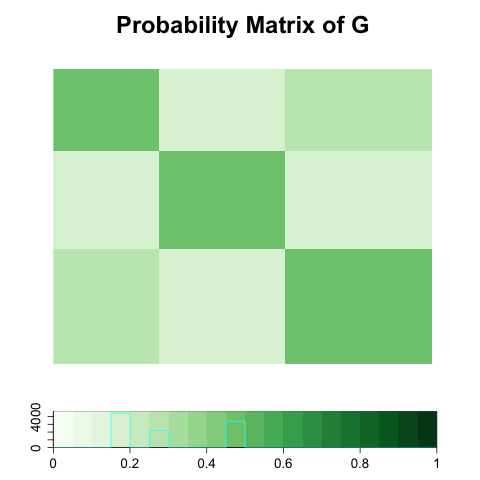
\includegraphics[width=1.7in]{../Figure/pmat.png}
	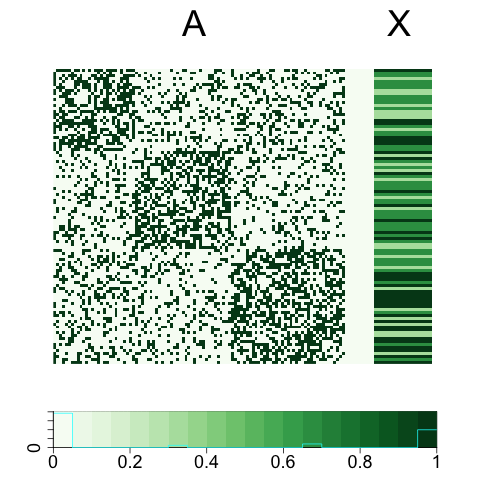
\includegraphics[width=1.7in]{../Figure/Amat.png}
	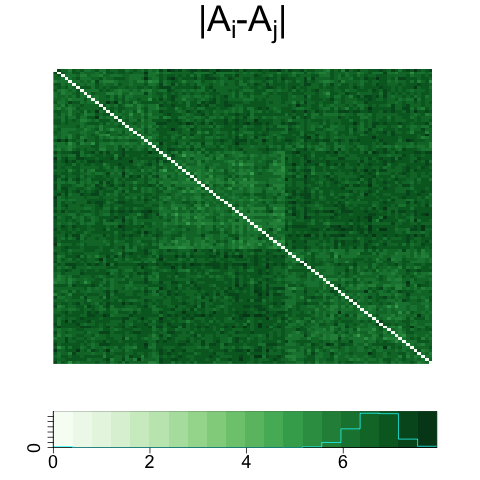
\includegraphics[width=1.7in]{../Figure/distA.png}
	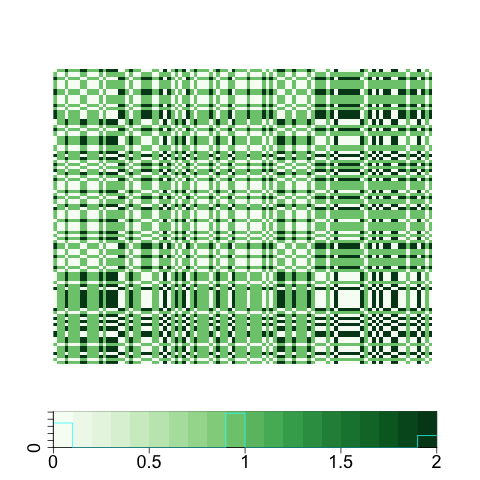
\includegraphics[width=1.7in]{../Figure/distX.png}
	\caption{Population probability distribution and realized values of $A$ and $X$ (scaled by 1/3) in the left two panels. Euclidean distance applied to realized $A$ and $X$ are presented in the right two panels. Data generation follows Eq.~\ref{eq:Three}.}
	\label{fig:matrics}
\end{figure}	

A transition matrix $P$ is a new kernel of a Markov chain of which element $P[i,j]$ represents the probability of travel from Node $i$ to Node $j$ in one time step. A transition matrix $P = \{P[i,j] : i,j=1,...,n \}$ in a Markov chain on $\mathbf{G}$ is defined as below:
\begin{equation}
P[i,j] = A_{ij} \big/ \sum\limits_{j=1}^{n} A_{ij}.
\end{equation}
 A corresponding probability in $t$ step is given by the $t^{\mbox{th}}$ ($t \in \mathbb{N}$) power of $P$. Now we assume that diffusion process occurs within a given graph with this transition probability at each time step. Distance between a pair of nodes at each time is called \textit{diffusion distance}. That is we have distance between every pair of nodes throughout diffusion process. How to derive diffusion distance over a directed network or weighted network is provided in \cite{tang2010graph}. Other than a transition matrix, we need a stationary probability $\mathbf{\pi} = \{\pi(1), \pi(2), ... , \pi(n) \}$ of which $\pi(i)$ represents the probability that the diffusion process in the end is stuck in Node $i$ regardless of the starting state. In our setting, $\pi(i)$ is assumed to be proportional to the degree of Node $i$, i.e. $\pi(i) = \sum\limits_{j=1}^{n} A_{ij} \big/ \sum\limits_{i=1}^{n}\sum\limits_{j=1}^{n} A_{ij}$ ($i=1,2,..., n$).  For each time point $t \in \mathbb{N}$, we can define a diffusion distance at time $t$, $C_{t}$:	
 \begin{equation}
 \label{eq:diffusion}
 \begin{split}
 C^2_{t}[i,j] & = \sum\limits_{w =1}^{n} \big( P^{t}[i,w] - P^{t}[j,w]  \big)^{2} \frac{1}{\pi(w)} = \sum\limits_{w=1}^{n} \left(  \frac{P^{t}[i,w]}{\sqrt{\pi(w)}} - \frac{P^{t}[j,w]}{\sqrt{\pi(w)}}   \right)^2 \\ & = \parallel P^{t}[i, \cdot] - P^{t}[j, \cdot]  \parallel^2_{L^{2}(\mathbf{G}, d\mu / \pi)  } \quad i,j = 1,2, \ldots , n
 \end{split}
 \end{equation}

\begin{figure}[H]
	\centering
	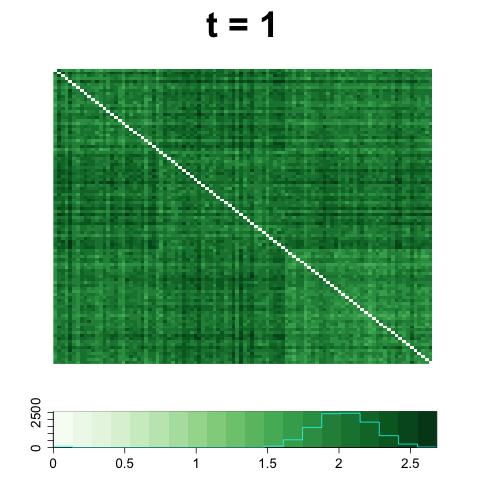
\includegraphics[width=1.7in]{../Figure/Dx1.png}
	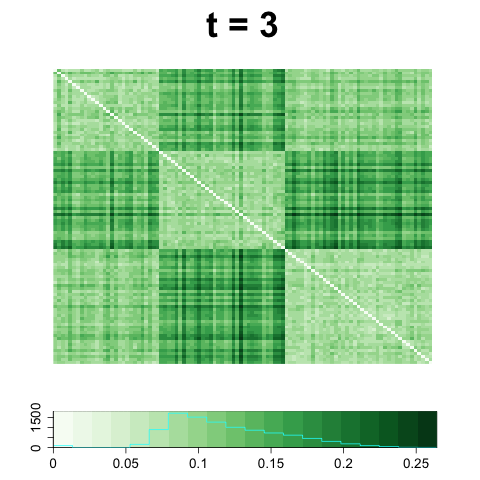
\includegraphics[width=1.7in]{../Figure/Dx3.png}
	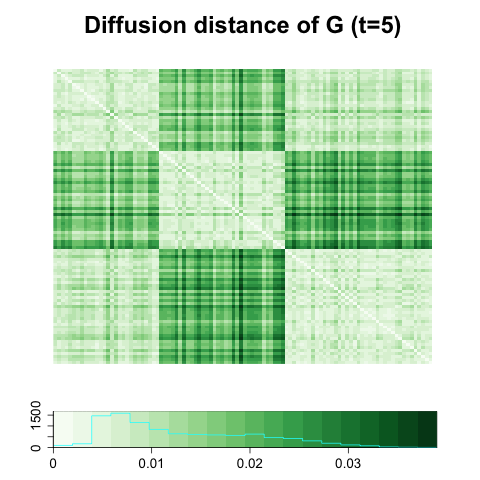
\includegraphics[width=1.7in]{../Figure/Dx5.png}
	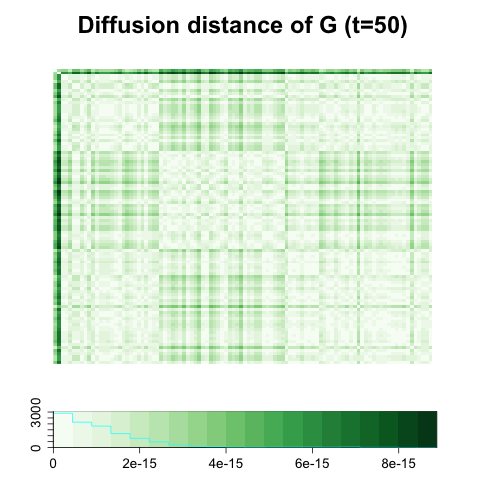
\includegraphics[width=1.7in]{../Figure/Dx50.png}
	\caption{Diffusion distance, i.e. Euclidean distance of diffusion maps at $t=1$, $t=3$, $t=5$, and $t=50$ of sample graph $G$ from Stochastic Block Model provided in simulation (Eq.~\ref{eq:Three}).}
	\label{fig:diffusions}
\end{figure}	
As diffusion time $t$ increases, distance matrix $C_{t}$ is more likely to take into account distance between two nodes which are relatively difficult to reach each other. Basically diffusion distance at fixed time $t$ measures the chance that we are likely to stay between Node i and Node j at $t$ step on our journey of all other possible paths. The higher this chance is, the smaller distance between two is. Depending on the distribution of network or graph, the optimal time $t$ when the diffusion distance is most correlated to the distance in terms of $\mathbf{X}$ can be different. If you see Figure~\ref{fig:diffusions}, difference between blocks in distance matrix at $t=3$ looks more distinct than that at $t=1$.  If you move to diffusion distance at $t=5$, you are able to distinguish every block in upper (or lower) diagonal. However if the propagation takes enough, e.g. at $t=50$, it becomes hard to detect the differences as nodes under the peer influence are at the end assimilated. On the other hand, compared to adjacent relation or geodesic distance, diffusion distance well reflects the connectivity since it takes into account every possible path between two nodes. Connectivity between two nodes is higher if we need to eliminate more number of nodes to disconnect these two. It is more robust measure to the unexpected edges than geodesic distance. Often a set of nodes with higher connectivity also have a higher propensity of having edges within this set and they are likely to form a cluster. This kind of cluster can be considered as a block in SBM framework. 
	
Diffusion distance of $\mathbf{G}$ defined as above can be represented via a spectral decomposition of its transition matrix $P$. That is, we can derive diffusion distance using its eigenvectors and eigenvalues \citep{coifman2006diffusion,lafon2006diffusion}. 
Recall that diffusion distance at time $t$, $C_{t}$, is a functional $L^2$ distance, weighted by 1/$\pi$ in Eq.~\ref{eq:diffusion}. If we transform the way to represent $C_{t}[i,j]$ slightly, we are able to obtain an orthonormal basis of $L^{2}(\mathbf{G}, d\mu / \pi)$ via eigenvalues and eigenvectors. 
Since an adjacency matrix $A$ does not guarantee a symmetric of $P$, define a symmetric kernel $Q = \Pi^{1/2} P \Pi^{-1/2}$, where $\Pi$ is a $n \times n$ diagonal matrix of which $i$th diagonal element is $\pi(i)$. Under compactness of $P$, $Q$ has a discrete set of real nonzero eigenvalues $\{ \lambda_{r} \}_{r = \{1,2,...,q \}}$ and a set of their corresponding orthonormal eigenvectors $\{ \psi_{r} \}_{r = \{1,2,..., q \} },$ i.e. $Q[i,j] = \sum\limits_{r=1}^{q} \lambda_{r} \psi_{r}(i) \psi_{r}(j)$ ($1 \leq q \leq n$).  Return to transition probability between Node $i$ and Node $j$,

\begin{equation}
\begin{split}
P[i,j] &  = \sqrt{\pi(j) / \pi(i) } Q[i,j] \\ &   = \sum\limits_{r=1}^{q} \lambda_{r} \big\{ \psi_{r}(i) / \sqrt{\pi(i)}  \big\} \big\{ \psi_{r}(j) \sqrt{\pi(j)} \big\}  \\ & : = \sum\limits_{r=1}^{q} \lambda_{r} \phi_{r}(i) \big\{ \psi_{r}(j) \sqrt{\pi(j)} \big\}
\end{split}
\end{equation}
where $\phi_{r}(i) := \psi_{r}(i) / \sqrt{\pi(i)}$. Then from $\sum\limits_{r=1}^{q} \psi^2_{r}(j) = 1$ for all $j \in \{1,2,...,n\}$, 
we can represent the diffusion distance as: 	
\begin{equation}
\begin{split}
C^2_{t}[i,j]  = \sum\limits_{r=1}^{n} \lambda^{2t}_{r} \big( \phi_{r} (i) - \phi_{r}(j)   \big)^2  
\end{split}
\end{equation}
That is,
\begin{equation}
C_{t}[i,j] = \parallel \mathbf{U}_{t}(i) - \mathbf{U}_{t}(j) \parallel
\end{equation}
where 
\begin{equation} 
\mathbf{U}_{t}(i) = \begin{pmatrix} \lambda^{t}_{1} \phi_{1}(i) \\ \lambda^{t}_{2} \phi_{2} (i)  \\ \vdots \\ \lambda^{t}_{q} \phi_{q}(i) \end{pmatrix} \in \mathbb{R}^{q}.
\end{equation}
Now we have  a family of $q$-variate($q \leq n$) diffusion maps $\{ \mathbf{U}_{t} \}_{t \in \mathbb{N}} $, of which Euclidean distance is diffusion distance. Embedding each node on Euclidean metric is a novel approach in testing independence on network space; there is no estimation nor model assumption involved. However there remains a matter of dependence between observed diffusion maps. 
	
\subsubsection{Properties of diffusion maps under exchangeable graphs}

We wish that diffusion maps are multivariate configuration of each node whose distance metric well reflects relative location on network space. However, due to the inter-correlated construction of $\mathbf{U}_{t}$, e.g. $i$th subject's diffusion depends on others in the given network, it is hard to say that the observed diffusion coordinates of $n$ subjects are independent observations. As for independence of $\mathbf{U}_{t}$, we need a concept of exchangeable graph explained in the earlier section. 

\begin{lemma}[Exchangeability and \textit{i.i.d} of $A$ in graphon]
	\label{lemma_graphon}
Assume that a connected, undirected and unweighted graph $\mathbf{G}$ is a graphon. Then 2-array of $\{ A_{ij} : i = 1,2,... ,n , i < j \}$ are  \textit{i.i.d} conditioning on some random link function $g : [0,1]^2 \rightarrow [0,1]$. Thus for fixed row (column) of $\mathbf{A}$, $\{ A_{i1}, A_{i2}, ... , A_{in} \} \setminus \{ A_{ii} \} $ , $i \in \{ 1,2,... , n \}$ are conditionally \textit{i.i.d} given a random link function $g$ or equivalently, its underlying distribution.  
\end{lemma}
From the above Lemma~\ref{lemma_graphon}, we can also prove exchangeability and conditional \textit{i.i.d} of diffusion maps family. 
	
\begin{lemma}[Exchangeability and \textit{i.i.d} of $\mathbf{U}_{t}$]
\label{main_lemma}
	Assume that a connected, undirected and unweighted graph $\mathbf{G}$ is a graphon, i.e. any exchangeable random graph from an infinite graph. Then its transition probability so thus diffusion maps at fixed time $t$ also exchangeable, conditional on link function of graph. Furthermore, by \textit{de Finetti's Theorem}~\ref{finetti}, such diffusion maps at $t$ are conditionally \textit{i.i.d} given its underlying distribution, specifically given random probability measure $\eta$ on $U_{t}$ and random link function $g$.    
\end{lemma}
	
Lemma~\ref{main_lemma} above furnishes us with \textit{i.i.d} one-parameter family of $\{ \mathbf{U}_{t} \}_{t \in \mathbb{N}}$ conditional on its underlying distribution. At each time of $t$,  $q$-variate diffusion coordinate assigns each node to its position in the network. Unfortunately this is a story only applied to exchangeable graph, which cannot be sparse. If we want to embed a set of nodes in sparse graphs, one more step of conditioning on point process $\mathbf{\theta}$ is needed, explained in Def.~$\ref{graphex}$.  
	
\begin{lemma}[Exchangeability and \textit{i.i.d} of $A$ in graphex]
\label{lemma_graphex}
Assume that a connected, undirected and unweighted graph $\mathbf{G}$ is a graphex. Then 2-array of $\{ A_{ij} : i = 1,2,... ,n , i < j \}$ are  \textit{i.i.d} conditioning on some random link function $g : [0,1]^2 \rightarrow [0,1]$ and unit-Poisson process $\mathbf{\theta}$. Thus for fixed row (column) of $\mathbf{A}$, $\{ A_{i1}, A_{i2}, ... , A_{in} \} \setminus \{ A_{ii} \} $ , $i \in \{ 1,2,... , n \}$ are conditionally \textit{i.i.d} on its underlying distribution, specifically conditioning on random link function $g$ and $\mathbf{\theta}$.  
\end{lemma}	

Similar to Lemma~\ref{main_lemma}, we are able to prove exchangeability of a transition matrix in graphex case, which extends to conditional \textit{i.i.d} of its diffusion maps. 

We have discussed embedding a vertex $v \in V(\mathbf{G})$ of exchangeable graph into its diffusion map of $\{\mathbf{U}_{t}\}$. As explained earlier, its Euclidean distance, which is ready to be applied to \texttt{MGC} statistics~\ref{eq:MGC}, takes into account all possible paths between every pair of nodes and measure the connectivity between them. Unlike in the other metrics in network, i.e. adjacency matrix or geodesic distance, triangle inequality holds in diffusion distance. Proof is provided in Appendix. Thanks to these properties of diffusion maps, we earn better interpretation of its Euclidean distance.
\begin{corollary}[Triangle inequality]
	\label{corollary1}
	For any fixed time $t (\in \mathbb{N})$, let $C_{t} : V(\mathbf{G})^2 \rightarrow \mathbb{R}_{+}$ be a diffusion distance defined on a pair of nodes in any connected and undirected graph $\mathbf{G}$. Then for any $v, w, z \in V(\mathbf{G})$,  
	\begin{equation}
	C_{t}(v,z) \leq C_{t}(v,w) + C_{t}(w,z)
	\end{equation}
\end{corollary}		
%%%%%%%%%%%%%%%%%%%%%%%%%%%%%%%%%%%%%%%%%%%%%%%
\subsubsection{One parameter family of test statistic}

If exchangeable observations are applicable to distance-based test statistics, e.g. \texttt{MGC}, we are almost able to dispense with obstacles in testing network independence.  Assume that we have a finite sample of infinitely exchangeable sequence $(\mathbf{X}, \mathbf{Y}) = \{ ( \mathbf{x}_{i}, \mathbf{y}_{i} ) : i=1,2, \ldots, n \}$, which is identically distributed as $(\mathbf{x}, \mathbf{y})$ with finite second moment. Then, by the properties of exchangeable sequences, there exist some random measure $\theta$ and $P$ such that : 
\begin{equation}
\begin{split}
& x_{i} | \theta  \overset{i.i.d}{\sim} \prod\limits_{i=1}^{n} f_{\mathbf{x}_{i} | \theta}(\mathbf{x}_{i} | \theta)  \\
& \int \prod\limits_{i=1}^{n} f_{ \mathbf{x}_{i} | \theta} ( \mathbf{x}_{i} | \theta ) P(d\theta)  \stackrel{d}{=}   \prod\limits_{i=1}^{n} f_{\mathbf{x}}(\mathbf{x}_{i})  \\
& \mathbf{x}_{i}   \overset{i.i.d}{\sim}  f_{X}(\mathbf{x})  \quad \mbox{ conditioning on the underlying distribution } f_{\mathbf{X}},
\end{split}
\label{eq:iid}
\end{equation}
where $f$ is a random, marginal distribution integrated over $\theta$; same arguments hold for exchangeable $\{ \mathbf{y}_{i}  \}$.

\begin{lemma}
	\label{lemma1}
   Under the above conditions, we have 
	\begin{eqnarray*}
		\mathcal{V}^{2}_{n}(\mathbf{X},\mathbf{Y}) &= \|g_{\mathbf{x},\mathbf{y}}^{n}(t,s)-g_{\mathbf{x}}^{n}(t)g_{\mathbf{y}}^{n}(s)\|^{2},
	\end{eqnarray*}
	where $g_{\cdot}^{n}$ is the empirical characteristic function based upon $\{(\mathbf{x}_{i},\mathbf{y}_{i}), i=1,2,...,n\}$, i.e., 
	\begin{eqnarray*}
		&g_{\mathbf{x},\mathbf{y}}^{n}(t,s) = \frac{1}{n}\sum_{j=1}^{n}\exp\{i \left\langle t,\mathbf{x}_{j} \right\rangle  +i \left\langle  s,\mathbf{y}_{j}\right\rangle \}, \\
		&g_{\mathbf{x}}^{n}(t) = \frac{1}{n}\sum_{j=1}^{n}\exp\{i \left\langle t,\mathbf{x}_{j}\right\rangle\}, \\
		&g_{\mathbf{y}}^{n}(s) = \frac{1}{n}\sum_{j=1}^{n}\exp\{i \left\langle s,\mathbf{y}_{j}\right\rangle\}.
	\end{eqnarray*}
\end{lemma}

\begin{lemma}
	\label{lemma2}
We have 
	\begin{eqnarray}
		\mathcal{V}_{n}^{2}(\mathbf{X},\mathbf{Y}) &\longrightarrow \mathcal{V}^{2}(\mathbf{x},\mathbf{y}) \quad \quad \mbox{ as } n \rightarrow \infty
	\label{eq:conv1}
	\end{eqnarray}
where $\mathcal{V}^{2} (\mathbf{x},\mathbf{y}) := \| g_{\mathbf{x},\mathbf{y}}(t,s) - g_{\mathbf{x}}(t) g_{\mathbf{y}}(s) \|^2$, and $g_{\cdot}$ is a characteristic function, e.g., $g_{\mathbf{x},\mathbf{y}}(t,s) = E\{\exp\{i \left\langle t,\mathbf{x} \right\rangle  +i \left\langle  s,\mathbf{y}\right\rangle \}\}$.
	It follows that 
	\begin{eqnarray}
		\mathcal{V}_{n}^{2}(\mathbf{X},\mathbf{Y}) &\rightarrow 0 \quad \mbox{ as } n \rightarrow \infty
		\label{eq:conv2}
	\end{eqnarray}
	if and only if $g_{\mathbf{x},\mathbf{y}}(t,s) = g_{\mathbf{x}}(t) g_{\mathbf{y}}(s)$, i.e., $\mathbf{x}$ is independent of $\mathbf{y}$.
\end{lemma}
Lemma~\ref{lemma1} and its following Lemma~\ref{lemma2} facilitate the use of distance correlation while satisfying \textit{Theorem 2} in \cite{szekely2007measuring}.  

\begin{theorem}
	Suppose that we are given $n$ pairs of exchangeable observations $(\mathbf{X}, \mathbf{Y}) = \{  (\mathbf{x}_{i}, \mathbf{y}_{i} ), i = 1,2, \ldots, n \}$ having finite second moment. Assume $\mathbf{x}_{i} \overset{i.i.d}{\sim} \mathbf{x}$ and $\mathbf{y}_{i} \overset{i.i.d}{\sim} \mathbf{y}, i = 1,2, \ldots, n$. Then
	\begin{eqnarray}
		\mathcal{V}_{n}^{2}(\mathbf{X},\mathbf{Y}) &\longrightarrow 0 \quad \mbox{ as } n \rightarrow \infty
	\end{eqnarray}	
	\textit{if and only if} $\mathbf{x}$ is independent of $\mathbf{y}$. Moreover, \texttt{dCorr} and \texttt{MGC} are consistent for testing dependence between $\mathbf{x}$ and $\mathbf{y}$, i.e., the testing power converges to $1$ asymptotically for any dependency of finite moments.
	\label{theoremMain}
\end{theorem}

Note that if $\{ \mathbf{x}_{i} : i = 1,2,\ldots, n \}$ are \textit{i.i.d}, they are exchangeable. thus estimated latent factors, which are assumed \textit{i.i.d} by \cite{fosdick2015testing} can also be applied to Theorem~\ref{theoremMain}. We already have shown that even under undirected network, diffusion maps remain exchangeable at each diffusion time point $t$. 

\begin{theorem}
	\label{theorem2}
	\texttt{MGC} is consistent in testing network independence with any exchangeable graph metric and nodal attributes, in particular testing independence between underlying distribution of diffusion maps and nodal attributes $\{ ( \mathbf{u}_{t},  \mathbf{x}  ) : i =1,2, \ldots , n \}$.
	\begin{equation}
	H_{0}  \quad : \quad f_{\mathbf{U}^{(t)} \cdot \mathbf{X}  }  = f_{\mathbf{U^{(t)}}} \cdot f_{\mathbf{X}}
	\label{eq:hypothesis}
	\end{equation}
	 In particular, the consistency also holds for the estimated latent positions and adjacency matrix of directed network.
\end{theorem}
		
 Underlying distribution of $\mathbf{U}_{t}$, i.e. $\iint  f_{\mathbf{U}_t} \big( \eta, g \big) P(d \eta) P(dg) = f_{\mathbf{U}^{(t)} } (\mathbf{u})$, given a link function $g$ and a random probability measure $\eta_{t}$ of $\mathbf{U}_t$ has been introduced to draw $\textit{i.i.d}$ from exchangeability. Since a family of diffusion maps, $\{ \mathbf{U}_{t} \}_{t \in \mathbb{N}}$ provides a configuration of every node in $\mathbf{G},$ the above hypothesis implies testing independence between the configuration of nodes in network space and in attribute space at each time of diffusion given the underlying distribution of $\mathbf{U}$.	
We are not going to state otherwise but if you assume to be given a unit-Poisson process $\{ \theta_{i} \}_{i=1}^{n}$, you can lead to the same results for sparse graphex as Theorem~\ref{theoremMain}. Even though we are not able to present testing results in \textit{all} alternatives, in the following section a few examples of sparse networks as well as exchangeable networks will guide you when and why our proposing method performs better than others. 

\subsubsection{Each node's contribution to dependency measure}

In the presence of nonlinear dependency or local (in)dependency, some nodes often exerts more reliance on their attributes than the others since the amount of dependence is not consistent over a set of nodes. Like other node-specific measure of its importance, e.g. centrality, each node's leverage on dependency measure can be of interest. Here we actually quantify each node's contribution to \texttt{MGC} statistic so that we know how much its location on network space and its attributes are correlated.
Let $(k^{*}, l^{*})$ be the optimal neighborhood choice in distance matrix $(C, D)$.  Denote the contribution of node $v \in V(G)$ to the testing statistic by  $c(\cdot) : v \rightarrow \mathbb{R}$. 
\begin{equation}
\label{contribution}
c(v) = \frac{1}{2 n^2} \sum\limits_{j=1}^{n} \left\{     \tilde{C}_{v j} \tilde{D}_{v j} I \big(  r (C_{v j}) \leq k^{*}  \big) I \big( r (D_{ v j }) \leq l^{*} \big) + \tilde{C}_{j v} \tilde{D}_{j v} I \big(  r (C_{j v}) \leq k^{*}  \big) I \big( r (D_{j v}) \leq l^{*} \big) \right\} 
\end{equation}

%%%%%%%%%%%%%%%%%%%%%%%%%%%%%%%%%%%%%%%%%%%%%%%%%%%%%%%%%%%%%%%%
\section{Simulation Study}
\label{sec:sim}
	
In simulation studies presented in this paper, we make a comparison between empirical testing power across various multivariate independence test statistics: \texttt{MGC}, \texttt{dCorr}(\texttt{mCorr}), Heller-Heller-Gorfine (\texttt{HHG}) \citep{heller2012consistent}, and likelihood ratio test of Fosdick and Hoff (\texttt{FH}). For computing statistical power, we used type I error $\alpha = 0.05$ and obtain p-values of each sample network via permutations. For fair comparison between these testing methods, we also present an additive model of latent factors, which is mostly targeted by \texttt{FH}.  All the simulation models are illustrated by joint distribution of adjacent matrix $\mathbf{A}$, nodal attributes $\mathbf{X}$, and latent variable $\mathbf{Z}$, which explains dependence structure between $\mathbf{A}$ and $\mathbf{X}$. 
\begin{equation}
\begin{split}
f(\mathbf{A}, \mathbf{X}, \mathbf{Z}) & = f_{A | Z}(\mathbf{A} | \mathbf{Z}) \cdot f_{Z | X}(\mathbf{Z} | \mathbf{X}) \cdot f_{X}(\mathbf{X}) 
\\ & = f_{A | Z}(\mathbf{A} | \mathbf{Z}) \cdot  f_{X | Z}(\mathbf{X} | \mathbf{Z} ) \cdot f_{Z} (\mathbf{Z}) 
\end{split}
\label{eq:joint_model}
\end{equation}	
According to the joint model in Eq.~\ref{eq:joint_model}, edge distribution and nodal attributes are correlated only through a node-specific latent variable $\mathbf{Z}$ no matter whether $\mathbf{X}$ is modeled via $\mathbf{Z}$ or vice versa. 

For each simulated network, empirical power will be derived by comparing observed statistic to the empirical distribution under the null. One example of empirical distributions under both independence and dependence are shown in Figure~\ref{fig:density} where the vertical lines indicate 95$\%$ quantiles of the null.
\begin{figure}[H]
	\centering
	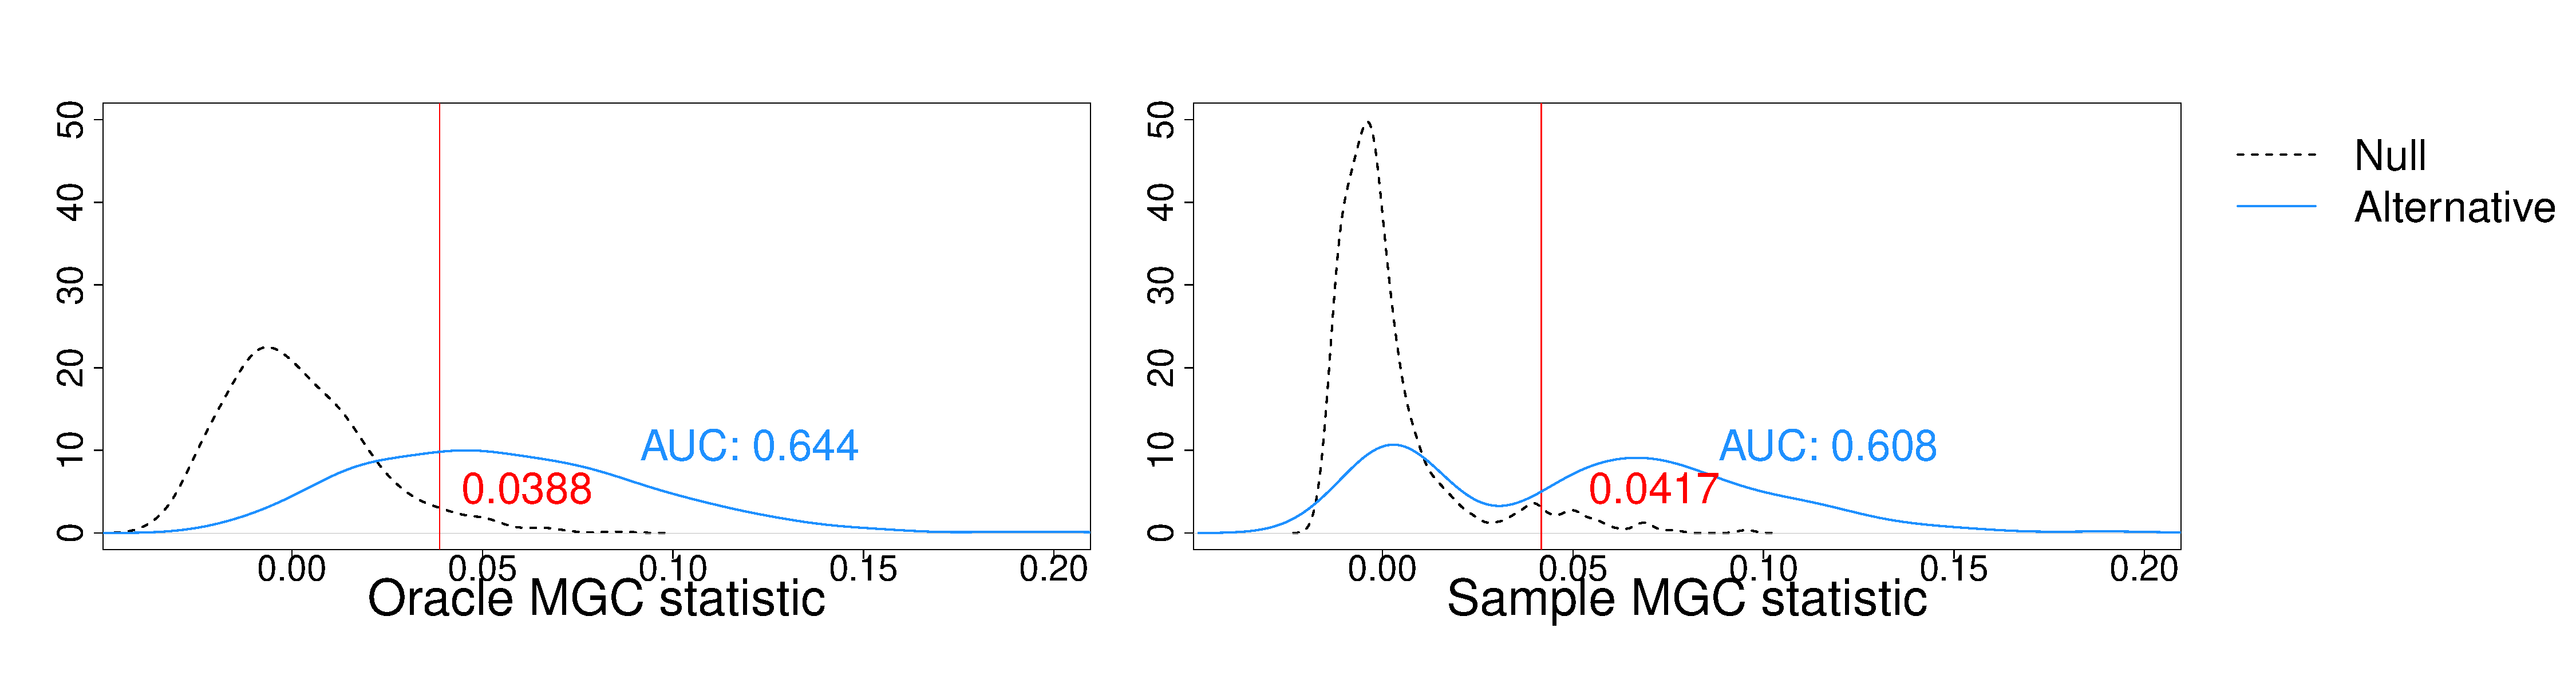
\includegraphics[width=7in]{../Figure/density.pdf}
	\caption{Statistics under null distribution and dependent distribution based on $M = 500$ independently generated SBM presented in Eq.~\ref{eq:Three}}
	\label{fig:density}
\end{figure}		
						
\subsection{Stochastic Block Model}

We already mentioned that Stochastic Block Model (SBM) is one of the most popular and also useful network generative model, especially as a tool for community detection \citep{karrer2011stochastic}. We first present the simplest SBM with $K = 2$ blocks where block affiliation for each node is correlated with its attributes $X$. Let us introduce block affiliation (latent) variable $Z \in \{ 0, 1 \}$. We set if $Z_{i}  = Z_{j}$, $A_{ij} = 0.4$ and $A_{ij} = 0.1$  otherwise so that nodes in the same block are more likely to be adjacent than nodes having different value of $Z$. 
For both cases, let $A_{ij} = A_{ji}$ and $A_{ii} = 0$, $i,j=1, \ldots n$. Figure~\ref{fig:twoSBM} and ~\ref{fig:Three} describe empirical power of \texttt{MGC}, \texttt{dCov}, and \texttt{HHG} based on diffusion distance, Euclidean distance of adjacent matrix and \texttt{FH}. In two block SBM, the performance of \texttt{MGC} is very similar to others while it is most superior in three block. This comparative advantage of \texttt{MGC} is attributed to its ability to capture non-linear dependence. Note that expectation of having edge between a pair of nodes is a monotonic function of (Euclidean) distance of their attributes in model~\ref{eq:twoSBM} but non-monotonic in model~\ref{eq:Three} as illustrate below. 
\begin{equation}
\begin{aligned}
E(A_{ij} | X_{i}, X_{j}) &  =  0.6 I(|X_{i} - X_{j}| = 0) + 0.4 I(|X_{i} - X_{i}| = 1)  \\
E(A_{ij} | X_{i}, X_{j}) & = 0.5 I(|X_{i} - X_{j}| = 0) + 0.2 I(|X_{i} - X_{j}| = 1) + 0.3 I(|X_{i} - X_{j}| = 2)
\end{aligned}
\end{equation}

\begin{figure}[h]
	\centering
	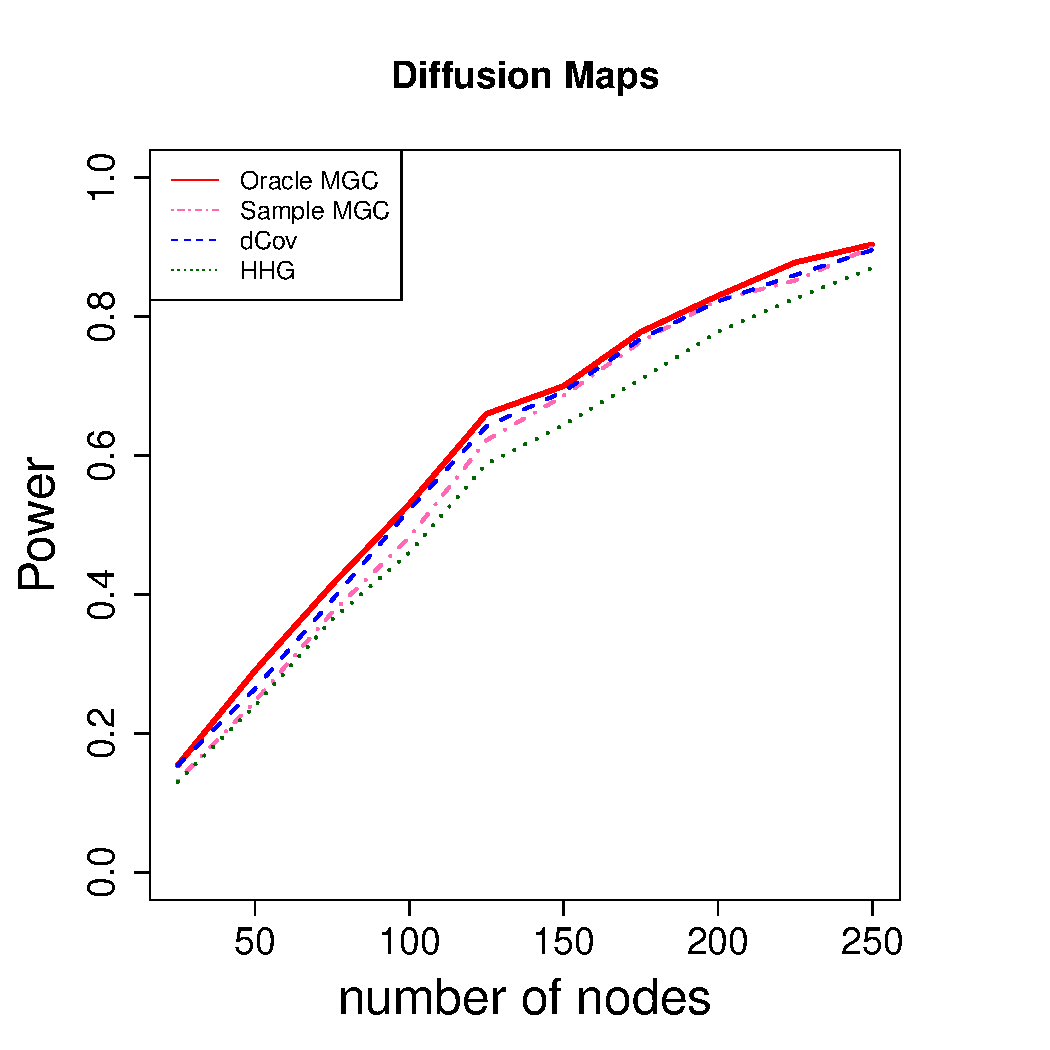
\includegraphics[width=7in]{../Figure/twoSBM.pdf}
	\caption{Empirical power based on $M = 500$ independently generated SBM presented in Eq.~\ref{eq:twoSBM} using diffusion maps (left) and Euclidean of adjacency matrix (middle)  and estimated latent position(right). The most right figure contains the results of \texttt{FH} test as well.}
		\label{fig:twoSBM}
\end{figure}
\begin{figure}[h]
	\centering
	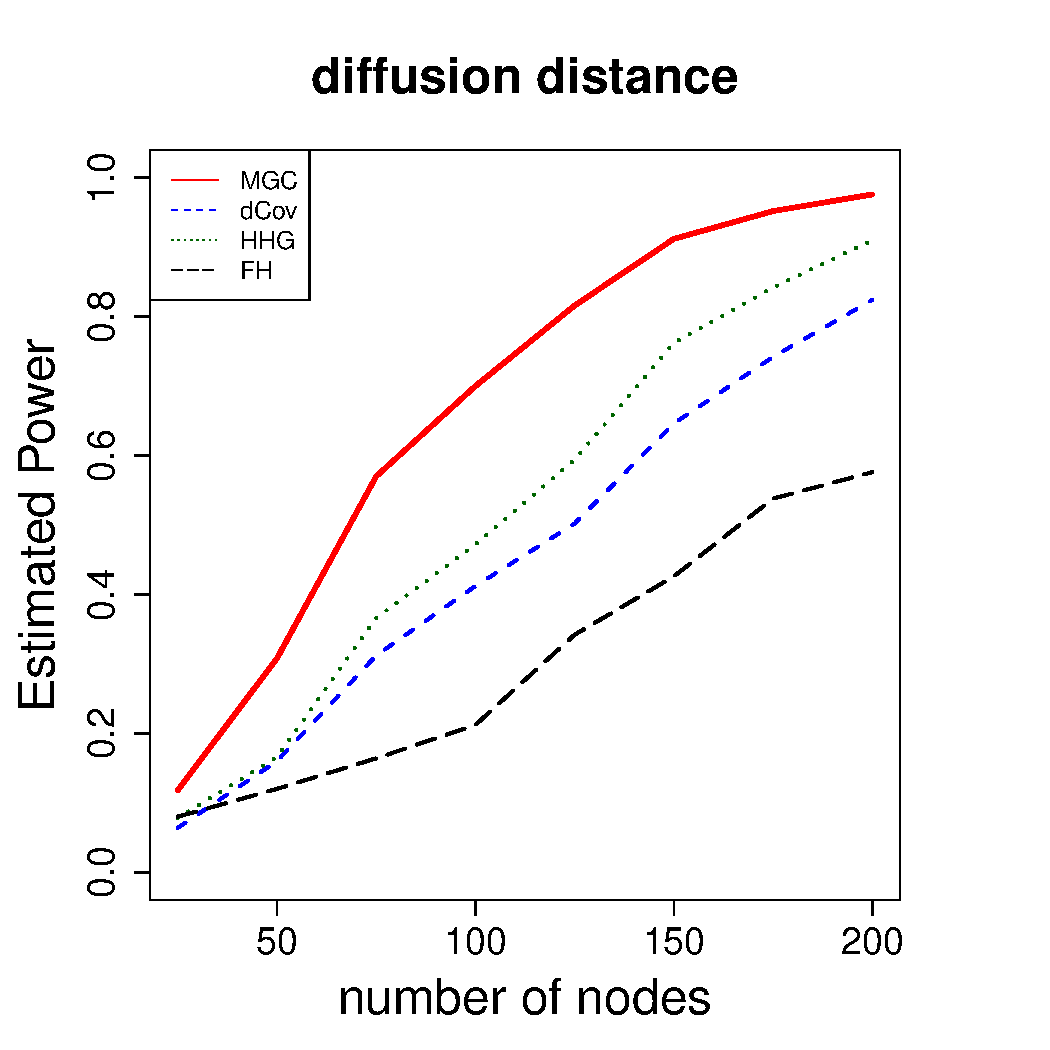
\includegraphics[width=7in]{../Figure/ThreeSBM.pdf}
	\caption{Empirical power based on $M = 500$ independently generated SBM presented in Eq.~\ref{eq:Three} using diffusion maps (left) and Euclidean of adjacency matrix (middle)  and estimated latent position(right). The most right figure contains the results of \texttt{FH} test as well.}
	\label{fig:Three}
\end{figure}	

Due to non-linear network dependence on attributes in the latter case, optimal neighborhood choice of $(k^{*}, l^{*})$ results in not global scale.  Figure~\ref{fig:ThreeSBM_power} demonstrates that neighborhood choice of $(k,l)$ in \texttt{MGC} statistic achieves its optimal in local scale. Roughly speaking, considering a pair of nodes in the nearest neighbor, in term of attribute values of $X$, e.g. (1,2) or (2,3), exhibits most significant dependence. When you only take into account these subsets of observations, you can actually represent $E(A_{ij} | X_{i}, X_{j})$ as a monotonic function of $|X_{i} - X_{j}|$ (equivalently $\parallel \mathbf{X}_{i} - \mathbf{X}_{j} \parallel$ in multivariate case). On the other hand, even in the three block SBM, If you set every pair of nodes in different blocks to have the same propensity of having edges, discrepancy between local and global scale of $(k,l)$ diminishes, which you can find in \textbf{Three Block SBM 2}, Appendix~\ref{sec:appendix}.

 To demonstrate better performance of local optimal scaled \texttt{MGC} over global scale of \texttt{dCorr} or \texttt{mCorr}, we control the amount of \textit{non-linear dependency} through changing the value of $\theta \in (0, 1)$. When $\theta > 0.2$, linear dependency of edge distribution upon nodal attribute $X$ is lost.
\begin{equation}
Power(\theta) = E(A_{ij} | X_{i}, X_{j}) = 0.5 I(|X_{i} - X_{j}| = 0) + 0.2 I(|X_{i} - X_{j}| = 1) + \theta I(|X_{i} - X_{j}| = 2)
\end{equation}

\begin{figure}[H]
	\centering
	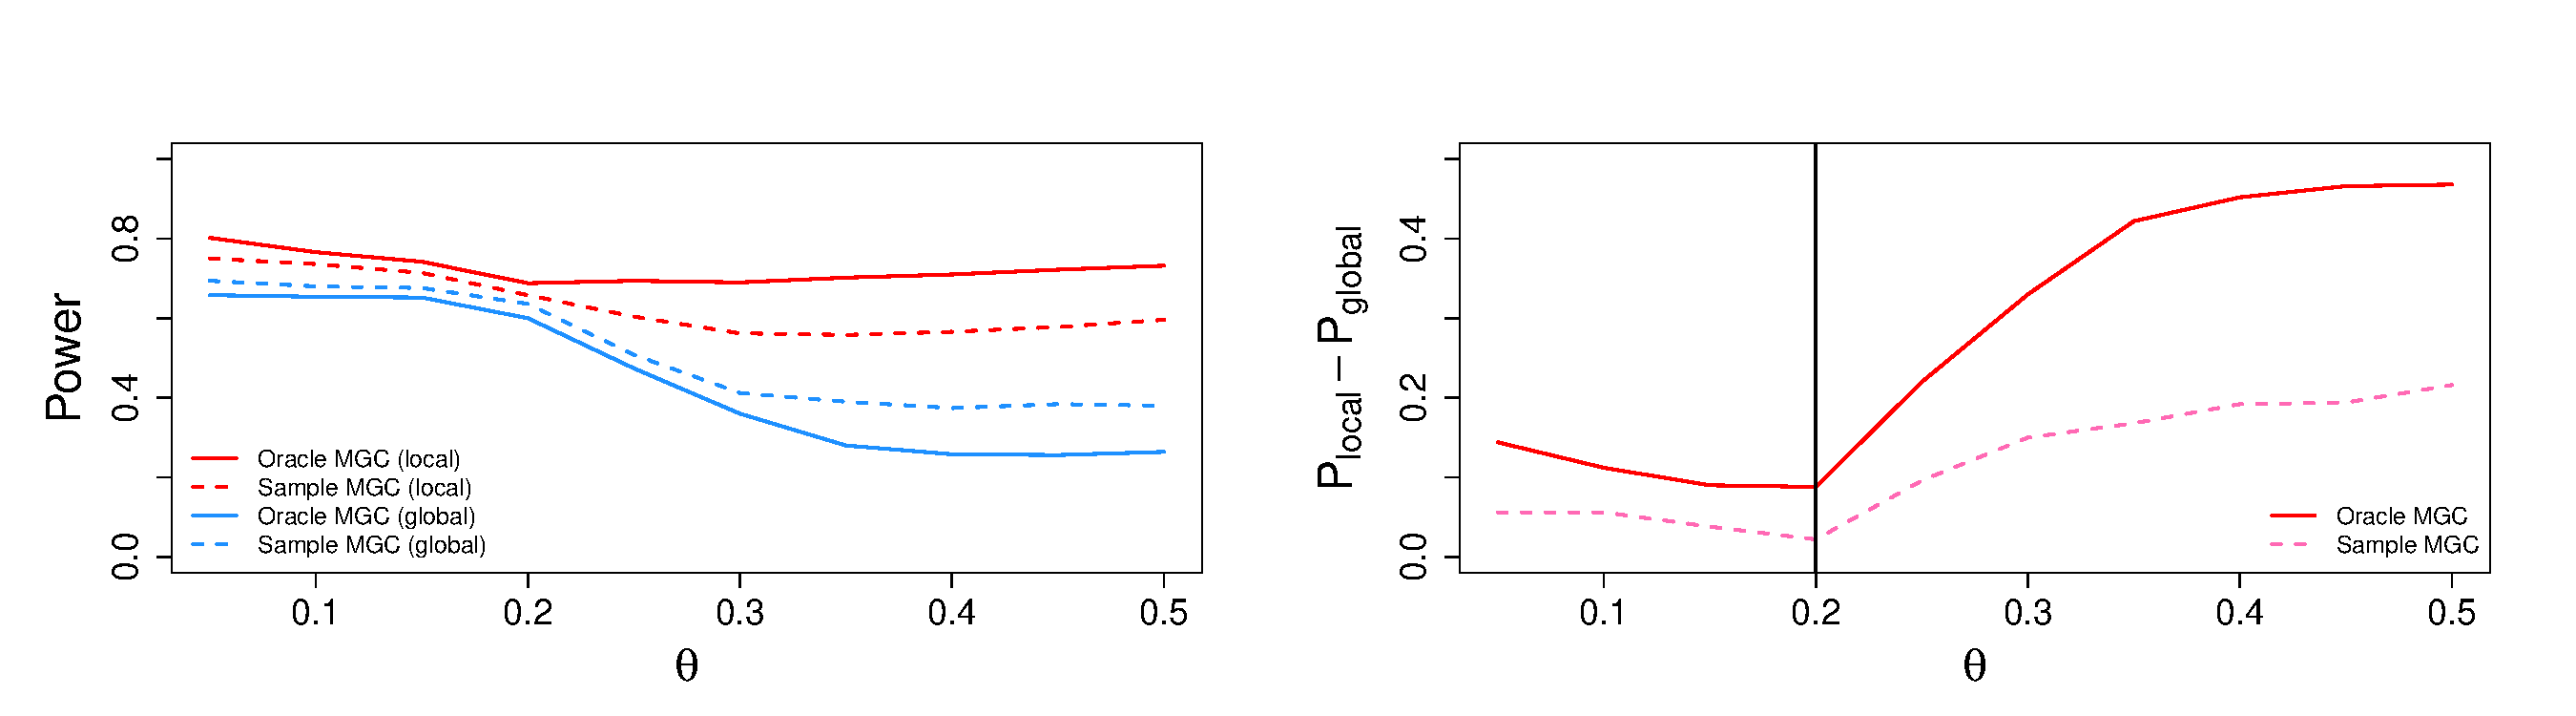
\includegraphics[width=7in]{../Figure/powerplot.pdf}
	\caption{Change of empirical power across $\theta$ in both local and global scale of distance correlation (left). Change of difference between these two powers in Oracle and Sample \texttt{MGC}. Superiority of optimal local scale become evident from $\theta > 0.2$, when distribution of edges have non-linear dependence on $X$.}
	\label{fig:powerplot}
\end{figure}
If you see Figure~\ref{fig:powerplot}, power of \texttt{dCorr} starts to drop from $\theta = 0.2$ while that of \texttt{MGC} almost stays clam, which implies \texttt{MGC} is significantly more sensitive to nonlinear dependency compared to \texttt{dCorr}.

\subsection{degree-corrected two block model}

Under SBM, we assumed that all nodes within the same block have the same expected degree. However, this block model is limited by homogeneous distribution within block and provides a poor fit to networks with hubs or highly varying node degrees within blocks or communities, which are common in practice. On the other hand, the Degree-Corrected Stochastic Block model (DCSBM) proposed by \cite{karrer2011stochastic} adds an additional set of parameter, often denoted by $\theta (>0)$, to control the node degrees. This model allows variation in node degrees within a block while preserving the overall block community structure. Consider two block SBM having same distribution of $X$ and $Z$ as model ~\ref{eq:twoSBM} but having different adjacency matrix with more variability induced by $\theta$.

\begin{figure}[h]
	\centering
	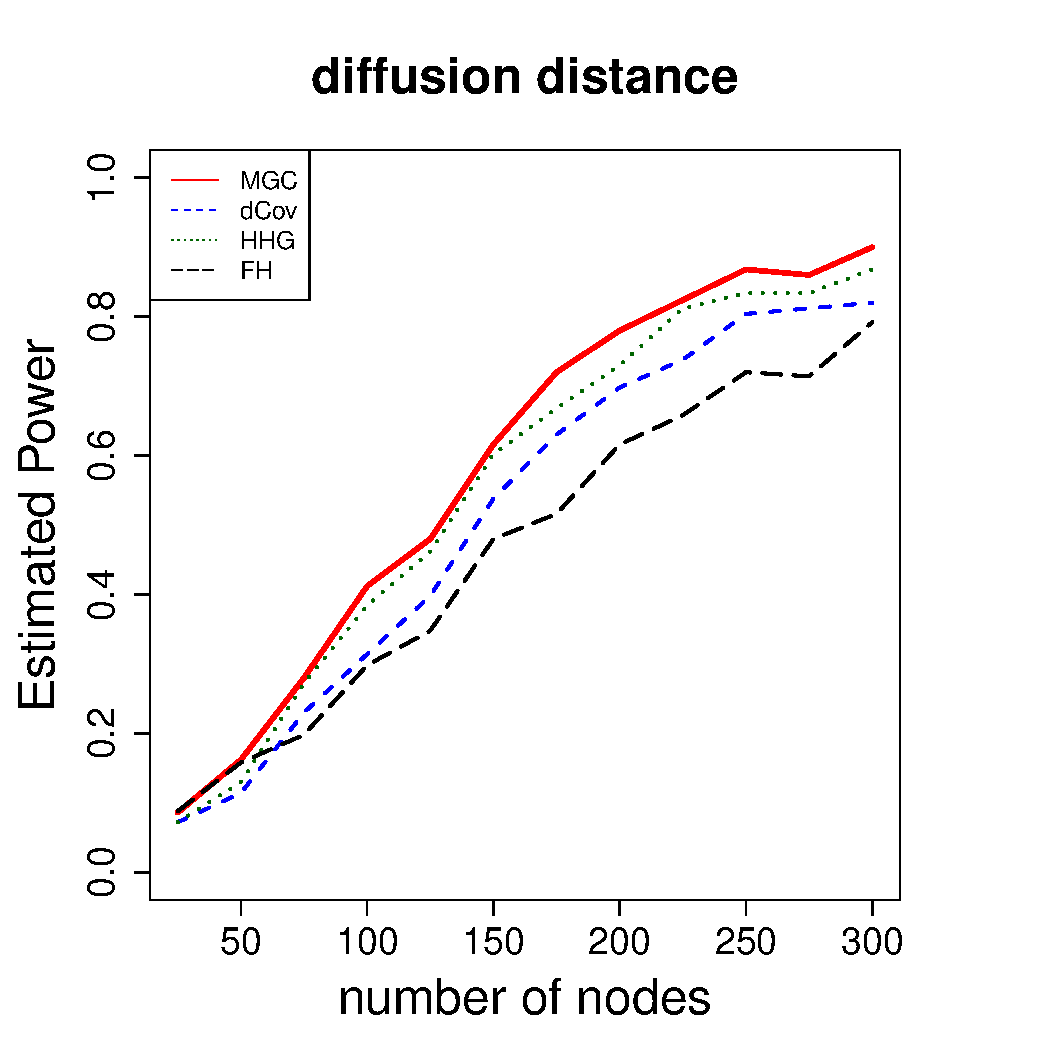
\includegraphics[width=7in]{../Figure/dcSBM.pdf}
	\caption{Empirical power based on $M = 500$ independently generated SBM presented in Eq.~\ref{eq:dcSBM} using diffusion maps (left) and Euclidean of adjacency matrix (middle)  and estimated latent position(right). The most right figure contains the results of \texttt{FH} test as well.}
		\label{fig:dcSBM}
\end{figure}	

As in the previous two block SBM, in this simulation scheme, we also observe monotonic edge distribution function of Euclidean distance. However its variance becomes inflated due to $\theta$ (model~\ref{eq:dcVariance}). If you see the testing results with Euclidean distance adjacency matrix in Figure~\ref{fig:dcSBM}, empirical power of \texttt{dCorr} or \texttt{HHG} shows far less than that of \texttt{MGC}. This might imply that multiscale statistic performs better than the other global ones even in the presence of variability of degree distribution. On the other hand, node-specific variable $\theta$ is captured by latent position estimation model \citep{fosdick2015testing} and \texttt{FH} test looks most sensitive in this case. (\textcolor{red}{why?}) 
	
\begin{equation}
\begin{aligned}
E(A_{ij} | X_{i}, X_{j}) &  =  0.2 I(|X_{i} - X_{j}| = 0) + 0.05 I(|X_{i} - X_{i}| = 1) \\
Var(A_{ij} | X_{i}, X_{j}) & = Var( Bern(0.2 \cdot \theta_{i} \theta_{j})) I(|X_{i} - X_{j}| = 0) +
Var( Bern(0.05 \cdot \theta_{i} \theta_{j}) ) I( |X_{i} - X_{j}| = 1) \\
& > Var(Bern(0.2)) I(|X_{i} - X_{j}| = 0) + Var(Bern(0.05)) I(|X_{i} - X_{j}| = 1).
\end{aligned}
\label{eq:dcVariance}
\end{equation}	
	
	
\subsection{Gaussian mixture model and SBM}

We only looked through univariate, binary value of nodal attributes $X$. Now let us consider multivariate, continuous nodal attributes $\mathbf{X}$, which specifically follows 2-dimensional Gaussian mixture model. 


	
\subsection{Additive and multiplicative graph model}

\begin{figure}[h]
	\centering
	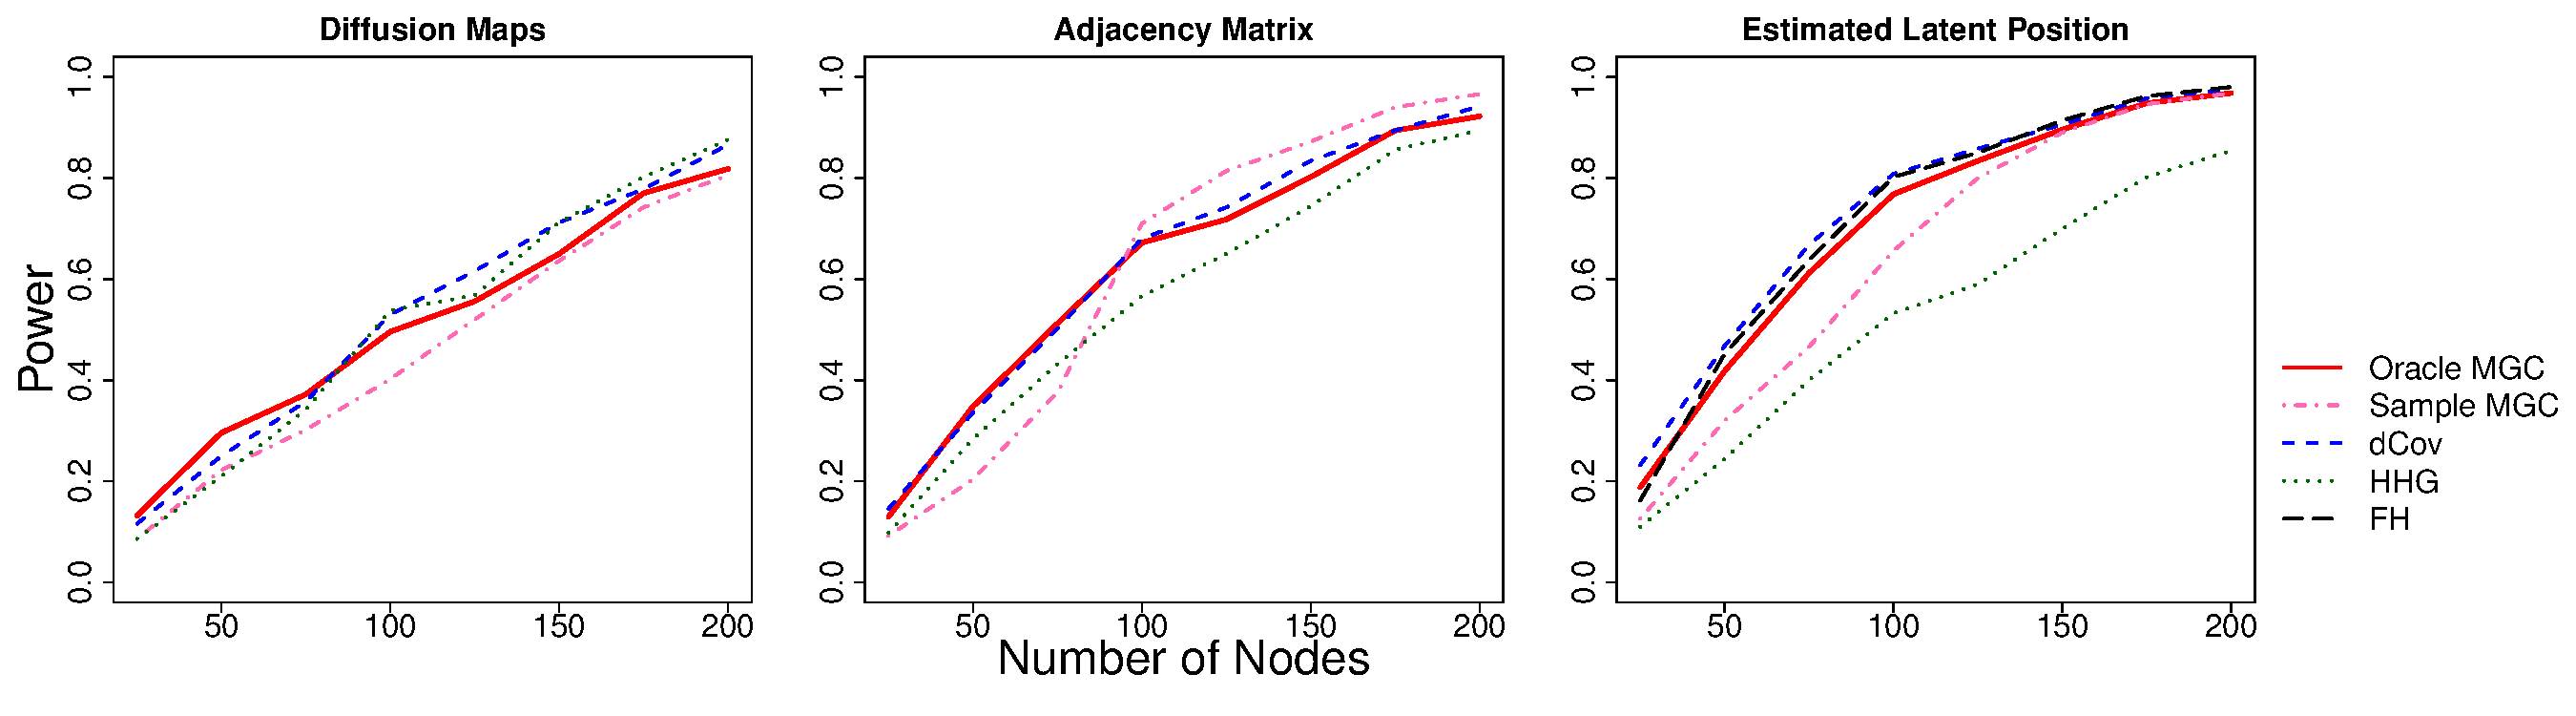
\includegraphics[width=7in]{../Figure/ame.pdf}
	\caption{Empirical power based on $M = 500$ independently generated SBM presented in Eq.~\ref{eq:ame} using diffusion maps (left) and Euclidean of adjacency matrix (middle)  and estimated latent position(right). The most right figure contains the results of \texttt{FH} test as well.}
		\label{fig:ame}
\end{figure}

\cite{hoff2002latent} proposed an approach of jointly modeling network and its attributes, where networks possess additional structure via sender-specific(or row-specific) and receiver-specific(or column-specific) latent factors. Whereas \cite{fosdick2015testing} embedded nodes into network factors assuming that additive an multiplicative network model is \textit{correct}, a family of diffusion maps are nonparametric version of embedding nodes into multivariate variable without losing any information on adjacent relationship. Thus in the model~\ref{eq:ame}, where logit of $A$ is an additive and multiplicative function of $\{\mathbf{w} \}$, their estimated factors would be very close to the truth, much closer than embedding made from diffusion maps. However we rarely see the network which is fitted to the model in reality. If you see that your observed network actually fits to their model, using network factors as independent observations from graph $\mathbf{G}$ and applying them to \texttt{MGC} performs not very worse than \texttt{FH} statistic (Fig.~\ref{fig:ame}).
Simply speaking, if network really fits well to additive and multiplicative model or we have basic knowledge about network model, then it becomes safe to use their node-specific additive factor $\{ a_{i} \}$ and multiplicative factor $\{ \mathbf{m}^{T}_{i} : \mathbf{m}_{i} \in \mathbb{R}^{k} \}$ in testing independence directly. Since they assume \textit{i.i.d} generative model for factors of each node, $\mathbf{F}_{i}$, i.e. $\mathbf{F}_{i} = \begin{pmatrix} a_{i} & \mathbf{m}^{T}_{i} \end{pmatrix} \overset{i.i.d}{\sim} MVNormal$, there is nothing wrong with applying \textit{MGC} using \textit{i.i.d} observations of $\{ \mathbf{F}_{i}, \mathbf{X}_{i} \}$.   
	
\subsection{Exchangeable graph on Poisson process}

\begin{figure}[H]
	\centering
	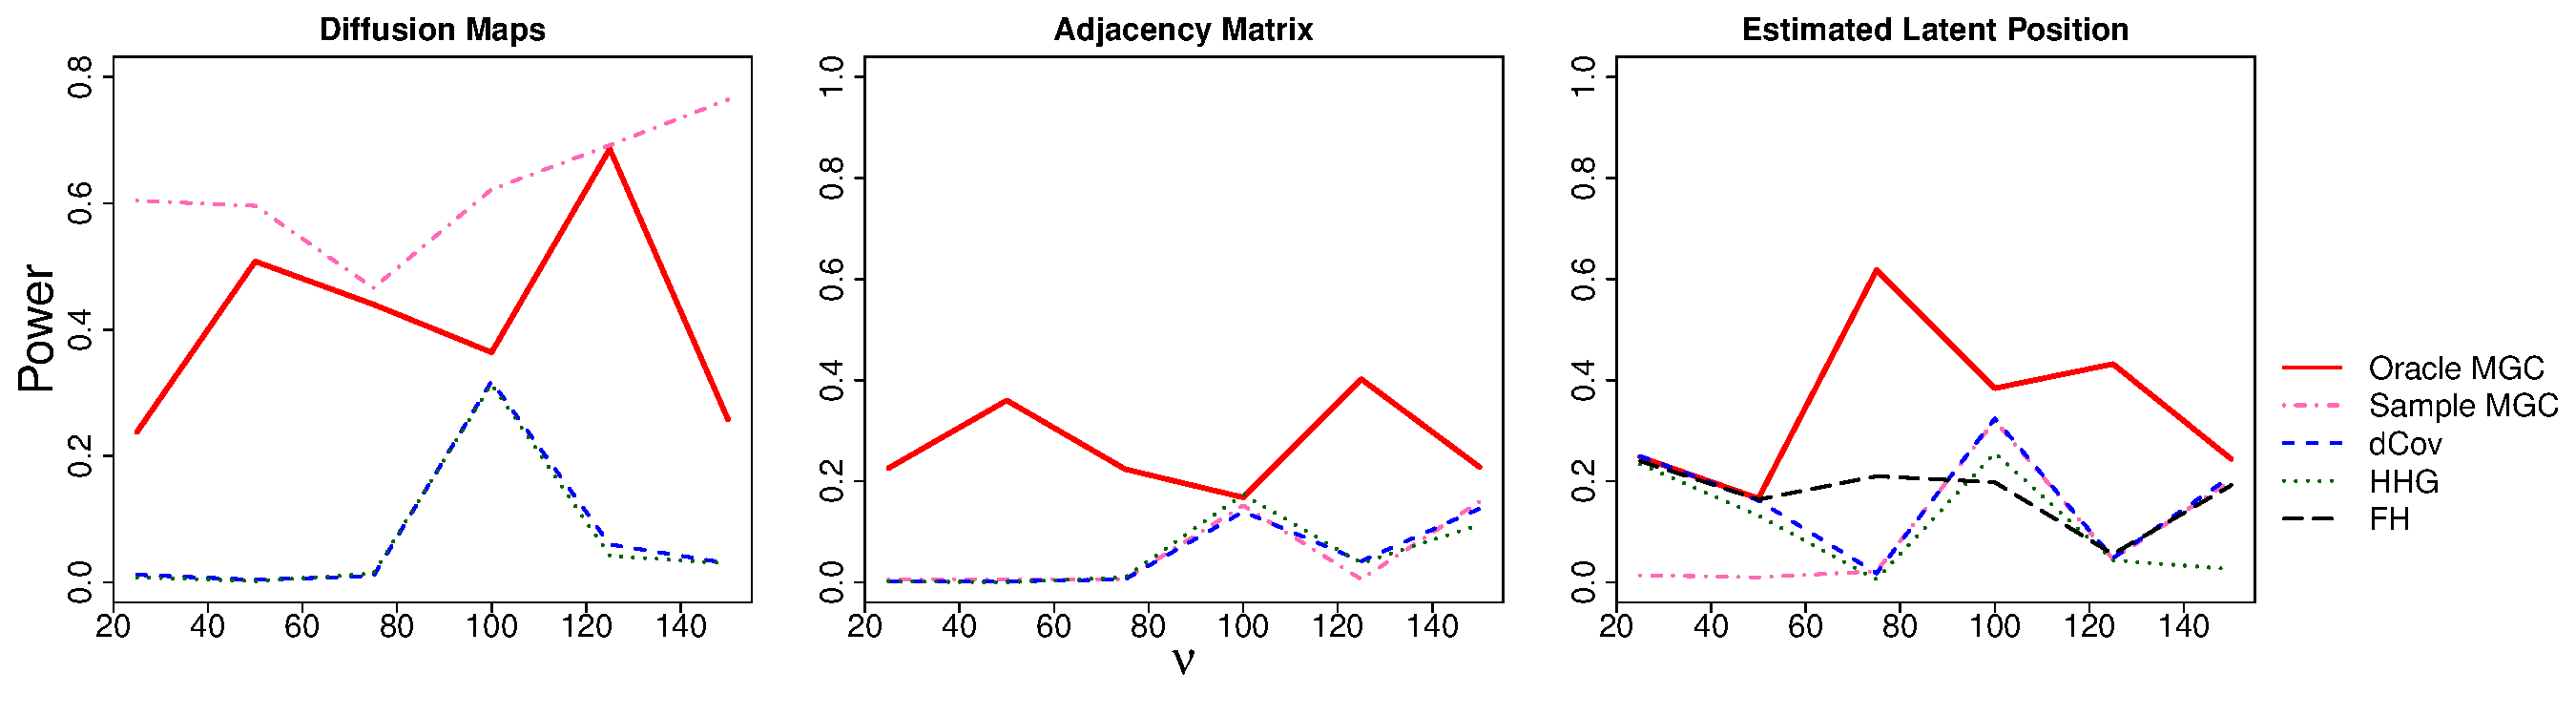
\includegraphics[width=7in]{../Figure/sparse.pdf}
	\caption{Empirical power based on $M = 500$ independently generated Poisson-processed exchangeable graphs presented in the model~\ref{eq:sparse} using diffusion maps (left), Euclidean of adjacency matrix (middle)  and estimated latent position(right). The most right figure contains the results of \texttt{FH} test as well.}
	\label{fig:sparse}
\end{figure}

We have discussed SBM and its derivative dcSBM in consideration of real network data. However an exchangeable network defined formally as Def.~\ref{exchangeability} still cannot embrace sparse network. Here we revisit the example of \textit{graphex} which is provided in \cite{veitch2015class}, which has power-law degree distribution (\ref{eq:sparse}). Simulation results in Figure~\ref{fig:sparse} does not show the linear power as $\nu$ increases since the variance of sample size ($N_{\nu}$) also increases as $\nu$ increases. In most cases, performance of \texttt{Oracle MGC} looks much better than the others and \texttt{Sample MGC} succeeds in catching up \texttt{Oracle MGC} under metrics of diffusion maps. 

%%%%%%%%%%%%%%%%%%%%%%%%%%%%%%%%%%%%%%%%%%%%%%%%%%%%%%%%%%%%%%%%
\section{Real Data Examples}
\label{sec:real}
	
\subsection{MRI}
	
\textcolor{red}{needs contexts}	
	
We look into one of the connected components with $n = 95$ nodes of whole disconnected network. 
	
$\{ \mathbf{U}_{t} \in \mathbb{R}^{95} \}_{t \in \mathbb{N}}$ $\mathbf{X} = (x,y,z) \in \mathbb{R}^{3}$
	
It turns out that $q=95$, i.e. full rank of transition matrix. In other words we are testing independence between 95-dimensional diffusion maps and 3-dimensional nodal attributes at each $t \in \mathbb{N}$.
	
	
test independence between brain network and its 3-dimensional locations; test independence between functional location and physical location. 
	
\begin{figure}[H]
	\centering
		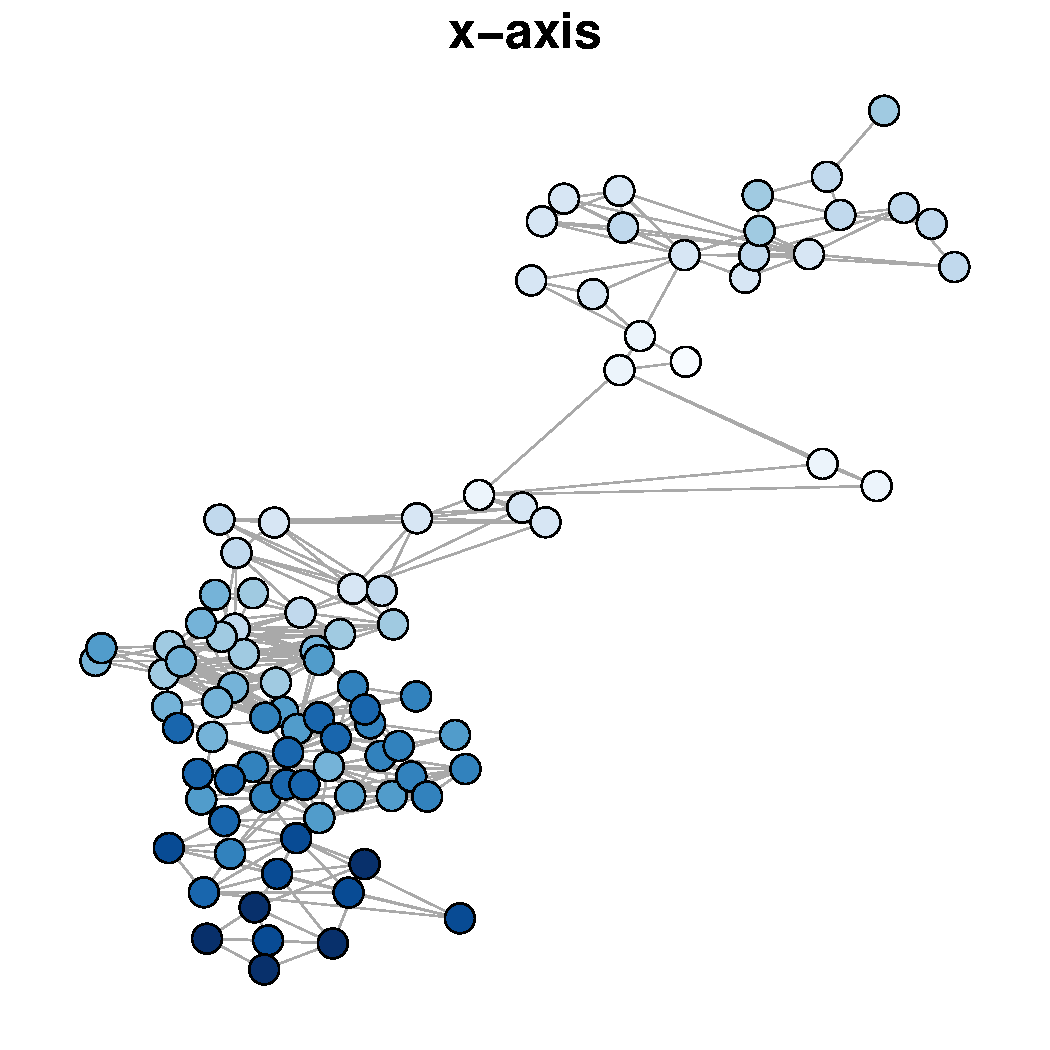
\includegraphics[width=1.5in]{../Figure/brain1_x.pdf}
		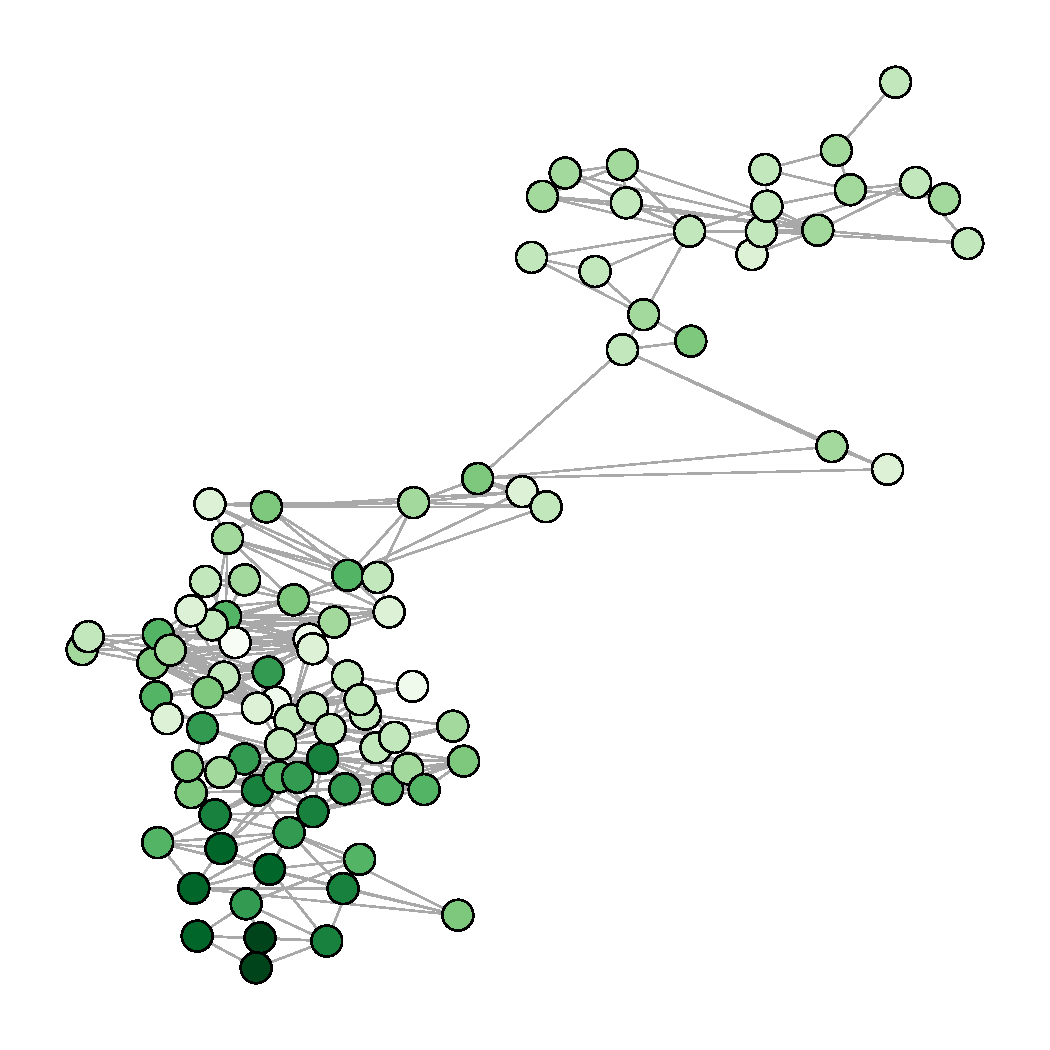
\includegraphics[width=1.5in]{../Figure/brain1_y.pdf}
		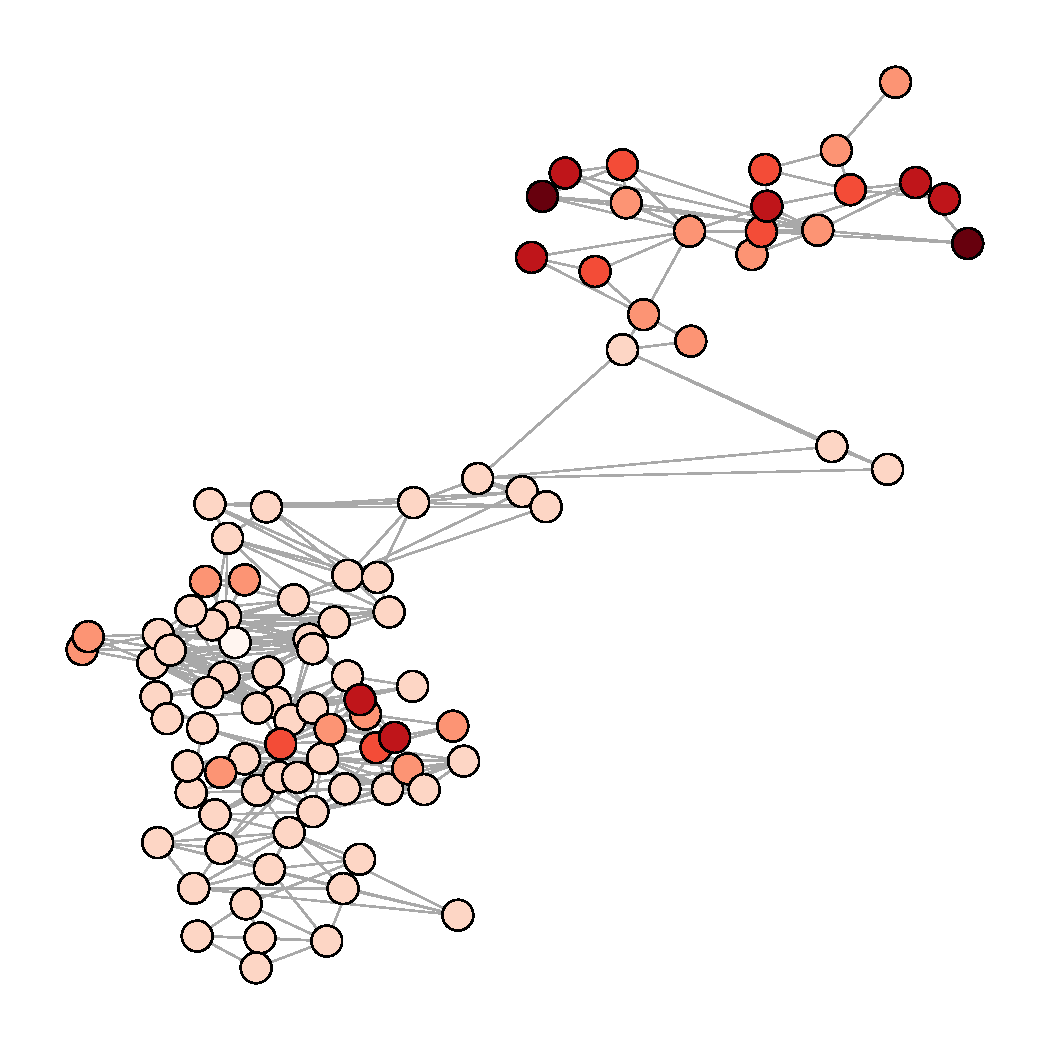
\includegraphics[width=1.5in]{../Figure/brain1_z.pdf}
		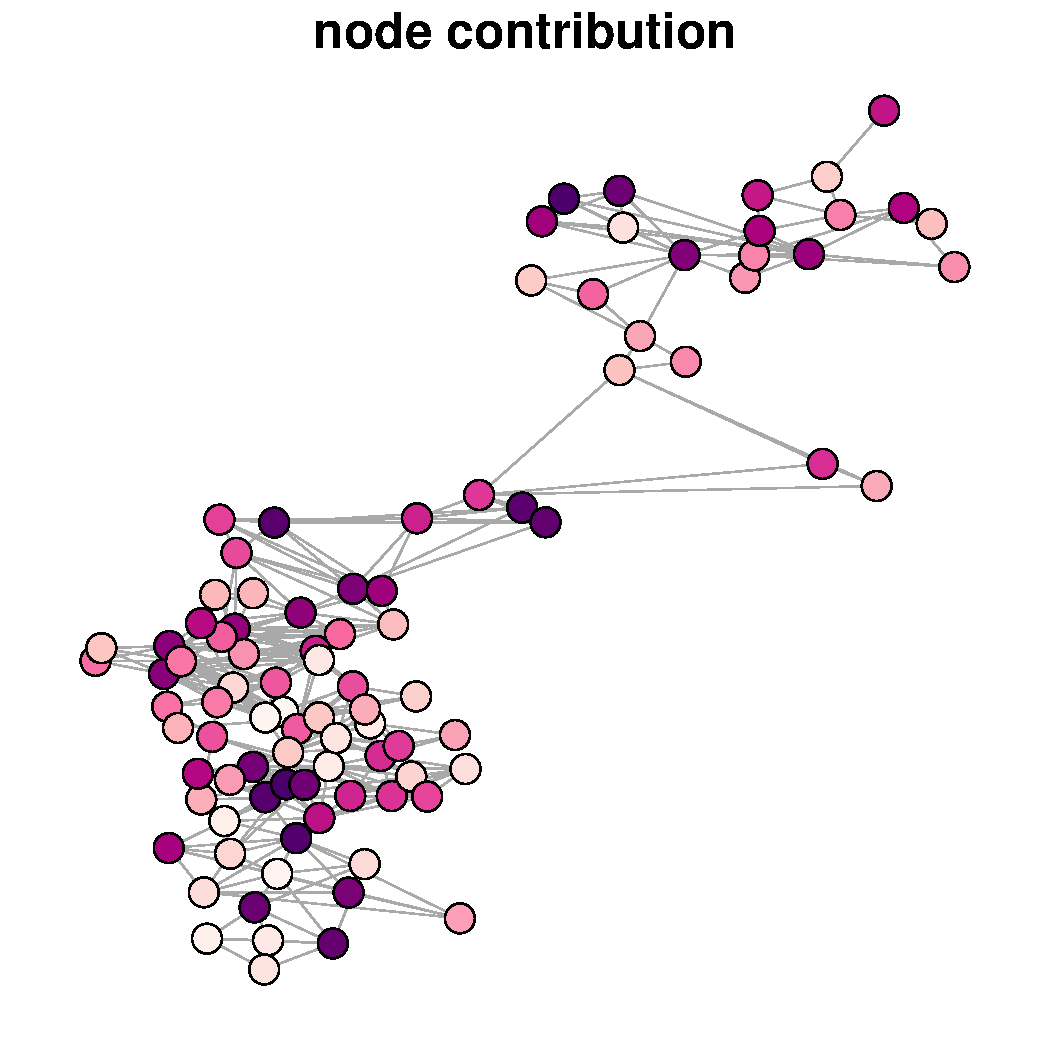
\includegraphics[width=1.5in]{../Figure/brain1_weight.pdf}
	\caption{Subnetwork of MRI network. Darker colored nodes indicate higher positioned node in terms of $x$-axis(left), $y$-axis(middle), and $z$-axis(right).}
		\label{fig:mri}
\end{figure}
	

%%%%%%%%%%%%%%%%%%%%%%%%%%%%%%%%%%%%%%%%%%%%%%%%%%%%%%%%%%%%%%%%
\section{Discussions}
\label{sec:discussion}
	
Throughout this study, we demonstrate that multiscale network test statistic to test  independence between network topology and its nodal attributes performs well in diverse settings, being supported by thorough theory on distance correlation and diffusion maps. These two tools are both specialized in detecting local and nonlinear dependence patterns, which other existing methods are lack of. However, testing independence is often the very first step in investigating relationship between network topology and nodal attributes in our interest. It is more likely that we want to know more than binary decision of rejecting or not rejecting the hypothesis. Multiscale test statistics attributed to both neighborhood choice $\{ (k,l)  \}$ and time spent in diffusion processes $\{ t \}$ provides us a hint on latent dependence structure as well. On the other hand, due to the ambiguousness of saying \textit{optimal}, our work has some limitations; we do not suggest any theoretically supported tools to select the \textit{optimal} time to obtain p-values of test statistics. Future research can be focused on restoring true dependence pattern or estimating \textit{optimal} scale from a family of statistics. In addition, obtaining a full family of statistics are also computationally infeasible; at every Markov process, we chose the optimal region of neighborhood. As an ad hoc, we selected optimal $t$ with highest power or lowest p-values from 1 to 10 for our simulation~\ref{sec:sim}.  Other than these computational issues, someone might be uncomfortable about being conditioned by a random function of $g$ and $\eta$.  However, we have to say that this is inevitable in order to argue sample properties of being \textit{i.i.d.}, which is also very conceptual and impossible to prove. Through conditioning diffusion maps $\{ \mathbf{U}_{t} \}$ by unknown network generative model $g(\cdot, \cdot)$ and also unknown diffusion process model $\eta(\cdot)$, we are finally able to assert that our observations are a fair sample eligible for test. 
	
Despite a few shortcomings listed above, a range of applications of \texttt{MNT} statistics and node-specific representation of network are very diverse. Especially multiscale version of test would be very useful when indirect networking through diffusion process is not ignorable or cluster membership significantly affects attributes. Furthermore even though we specifically constraint the statistic into testing independence between network and nodal attributes, we are able to implement independence testing of two networks with same size by inputting diffusion distance at each time point from each of network in Eq.~\ref{eq:MGC}. This type of test will be useful when we want to show a pair of networks are topologically or structurally independent. For example, we might wonder if network on \textit{Facebook} and network induced by club activity within class or school are independent or not; if DNA methylation network is correlated with gene expression network \citep{bartlett2014dna} so that the behavior of interest measured by DNA methylation network can be matched to that noticed by gene expression network, etc.  In a broad sense, we suggest a proper metric applied to network and justify its use in measuring correlations between \textit{network vs. attributes} or possibly \textit{network vs. network}. Even though we have fully presented procedures, e.g. testing on diffusion maps from $t=1$ to $t=10$  and obtaining a family of all local scales for each, depending on the previous knowledge or on the results of model fitting, you may shorten the steps as well. We also presented the case where additive and multiplicative models work pretty well and how to modify the statistic in this case. Likewise the application and variation of multiscale network test is almost limitless. 


 	
%%%%%%%%%%%%%%%%%%%%%%%%%%%%%%%%%%%%%%%%%%%%%%%%%%%%%%%%
\appendix
\section{appendix}
\label{sec:appendix}

\subsection{simulation schemes}

\begin{itemize}	
	\item \textbf{Two Block SBM}	
	%\begin{equation}
	\begin{equation}
	\begin{gathered}
	\begin{aligned}
	&	X_{i}  \overset{i.i.d}{\sim} f_{X}(x)  \stackrel{d}{=}  Bern(0.5), \quad   i = 1, \ldots , n \\ 
	&	Z_{i} | X_{i}   \overset{i.i.d}{\sim}    f_{Z|X}(z|x)  \stackrel{d}{=}  Bern(0.6) I( x = 0 ) +   Bern(0.4) I (x = 1), \quad  i = 1,\ldots,n  \\
	&	A_{ij} | Z_{i}, Z_{j}   \overset{i.i.d}{\sim}   f_{A|Z}(a_{ij} | z_{i}, z_{j}) \stackrel{d}{=}  Bern(0.4) I ( |z_{i} - z_{j}| = 0 )  + Bern(0.1) I(|z_{i} - z_{j}| > 0) \\ & \quad \quad \quad i < j, i,j=1, \ldots n 
	\end{aligned}
	\end{gathered}
	\label{eq:twoSBM}
	\end{equation} 
	
	%\end{equation}
	\item \textbf{Three Block SBM 1}
	\begin{equation}
	\label{eq:Three}
	\begin{gathered}
	\begin{aligned}
	&  X_{i} \overset{i.i.d}{\sim} f_{X}(x)   \stackrel{d}{=}  Multi(1/3, 1/3, 1/3), i = 1, \ldots , n \\ 
	&  Z_{i} | X_{i}  \overset{i.i.d}{\sim}    f_{Z|X}(z|x)  \stackrel{d}{=}   Multi(0.5, 0.25, 0.25) I( x = 1 ) +   Multi(0.25, 0.5, 0.25) I (x = 2)  \qquad  \\ & \quad \quad + Multi(0.25, 0.25, 0.5)I(x = 3), \quad  i = 1,\ldots,n  \\
	&  A_{ij} | Z_{i}, Z_{j}   \overset{i.i.d}{\sim}   f_{A|Z}(a_{ij} | z_{i}, z_{j}) \stackrel{d}{=}  Bern(0.5) I ( |z_{i} - z_{j}| = 0 )  + Bern(0.2) I(|z_{i} - z_{j}| = 1) \\ & \quad \quad + Bern(0.3) I (|z_{i} - z_{j}| = 2),  \quad i < j, i,j=1, \ldots n 
	\end{aligned}
	\end{gathered}
	\end{equation}
	
	\item \textbf{Degree-corrected SBM}
	\begin{equation}
	\label{eq:dcSBM}
	\begin{gathered}
	\begin{split}
	\theta_{i} \overset{i.i.d}{\sim} Uniform(0,2), i = 1, \ldots, n \\ 
	A_{ij} | \mathbf{Z}, \mathbf{\theta}   \overset{i.i.d}{\sim}   f_{A|Z, \theta}(a_{ij} | z_{i}, z_{j}, \theta_{i}, \theta_{j}) \stackrel{d}{=} & Bern(0.2 \cdot \theta_{i}\theta_{j}) I ( |z_{i} - z_{j}| = 0 )  + Bern(0.05 \cdot \theta_{i} \theta_{j} ) I(|z_{i} - z_{j}| = 1) 
	\end{split}
	\end{gathered}
	\end{equation}
	
	\item \textbf{Gaussian mixture model and SBM}
	\begin{equation}
		\label{eq:gaus}
		\begin{gathered}
		\begin{split}
		&Z_{i} \overset{i.i.d}{\sim}  f_{Z}(z) \stackrel{d}{=} Bern(0.5), i = 1, \ldots, n \\ 
		& \mathbf{X}_{i} | Z_{i} \overset{i.i.d}{\sim} f_{\mathbf{X}|Z}(\mathbf{x}|z) \stackrel{d}{=} (0.3+0.4z) \mathbf{N}_{1} + (0.7 - 0.4z) \mathbf{N}_{2} \\
		& A_{ij} | Z_{i}, Z_{j} \overset{i.i.d}{\sim} f_{A|Z} (a_{ij} | z_{i}, z_{j}) \stackrel{d}{=} Bern(0.4) I\big( |z_{i} - z_{j}| = 0 \big) + Bern(0.1 ) I(|z_{i} - z_{j}| > 0), \\
		& \quad \quad \quad  i < j, i,j =1,\ldots, n
		\end{split}
		\end{gathered}
	\end{equation}
	where $\mathbf{N}_{1} = \left(  \begin{pmatrix}  0 \\ 0 \end{pmatrix}, \begin{pmatrix} 1 & 0.5 \\ 0.5 & 1 \end{pmatrix}    \right)$ and $\mathbf{N}_{2} = \left(  \begin{pmatrix}  1 \\ -1 \end{pmatrix}, \begin{pmatrix} 1 & 0.5 \\ 0.5 & 1 \end{pmatrix}    \right)$.
	
	\item \textbf{Additive and Multiplicative Graph Model}
	\begin{equation}
		\label{eq:ame}
		\begin{gathered}
		\begin{aligned}
		&	Z_{i} \overset{i.i.d}{\sim} f_{Z}(z) \stackrel{d}{=} Uniform[0,1]. \quad i = 1, \ldots, n \\ 
		&	X_{i} | Z_{i} \overset{i.i.d}{\sim}  f_{Z|X}(z|x) \stackrel{d}{=}  Normal(Z_{i}, 1), \quad i= 1, \ldots, n \\
		&	A_{ij} | Z_{i}, Z_{j} \overset{i.i.d}{\sim}  f_{A|Z}(a_{ij} | z_{i}, z_{j}) \stackrel{d}{=}   Bern \big(  ( 1 - z_{i})^2 \times (1 - z_{j})^2    \big), \quad i < j, i,j = 1, \ldots, n
		\end{aligned}
		\end{gathered}
	\end{equation}
	
	\item \textbf{Exchangeable Graph on Poisson Process}
	
	\begin{eqnarray}
	\begin{gathered}
	\begin{split}
	N_{\nu} \overset{i.i.d}{\sim} f_{N}(n)   \stackrel{d}{=} Poi( c \nu)  &   \quad \quad &
	\vartheta_{i}  \overset{i.i.d}{\sim} f_{\vartheta} \stackrel{d}{=} Uniform[0,1] \\
	\theta_{i} \overset{i.i.d}{\sim} f_{\theta |  N_{\nu}} (\theta)     Uniform[0, \nu]  & \quad \quad  & X_{i}    \overset{ind}{\sim} f_{X | \vartheta}(x_{i}) \stackrel{d}{=} Normal \big( \vartheta_{i}, 4^2 \big)  \\ 
	(\theta_{i}, \theta_{j})  \overset{ind}{\sim} f_{ (\theta_{i}, \theta_{j})  | W, \vartheta} ( (\theta_{i}, \theta_{j}) ) \stackrel{d}{=}   Bernoulli \big( W\big( \vartheta_{i}, \vartheta_{j} \big) \big)  &  \quad \quad & A_{ij}  \stackrel{d}{=} (\theta_{i}, \theta_{j})
	\label{eq:sparse}
	\end{split}
	\end{gathered}	 
	\end{eqnarray}	
	where $c = 1$ and $W(\vartheta_{i}, \vartheta_{j} ) = (\vartheta_{i} + 1)^{-2} ( \vartheta_{j} + 1 )^{-2}$ or 0 if $\vartheta_{i} = \vartheta_{j}$. 
\end{itemize}

\textbf{Three Block SBM 2}
\begin{equation}
\begin{gathered}
\begin{aligned}
& X_{i} \overset{i.i.d}{\sim} f_{X}(x)   \stackrel{d}{=}  Multi(1/3, 1/3, 1/3), \quad i = 1, \ldots , n \\ & Z_{i} | X_{i}  \overset{i.i.d}{\sim}    f_{Z|X}(z|x)  \stackrel{d}{=}   Multi(0.5, 0.25, 0.25) I( x = 1 ) +   Multi(0.25, 0.5, 0.25) I (x = 2)   \\ &  \quad \quad + Multi(0.25, 0.25, 0.5), \quad  i = 1,\ldots,n  \\
& A_{ij} | Z_{i}, Z_{j}   \overset{i.i.d}{\sim}   f_{A|Z}(a_{ij} | z_{i}, z_{j})  \stackrel{d}{=} Bern(0.5) I ( |z_{i} - z_{j}| = 0 ) \\  &  \quad \quad + Bern(0.2) I(|z_{i} - z_{j}| > 1) \quad i < j, i,j=1, \ldots n \\ & A_{ji} = A_{ij} ;   A_{ii} = 0,   \quad  i,j=1, \ldots n
\end{aligned}
\end{gathered}
\label{eq:simplethree}
\end{equation}

\subsection{supplementary figures}

\begin{figure}[H]
	\centering
	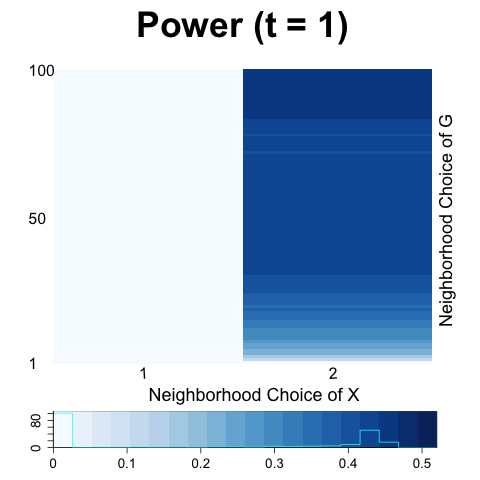
\includegraphics[width=2in]{../Figure/twoSBM_power1.png}
	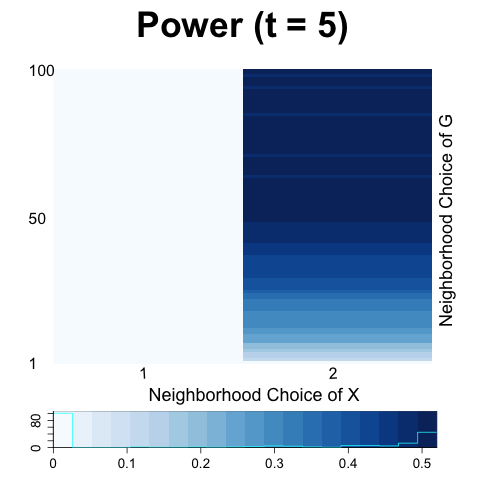
\includegraphics[width=2in]{../Figure/twoSBM_power5.png}
	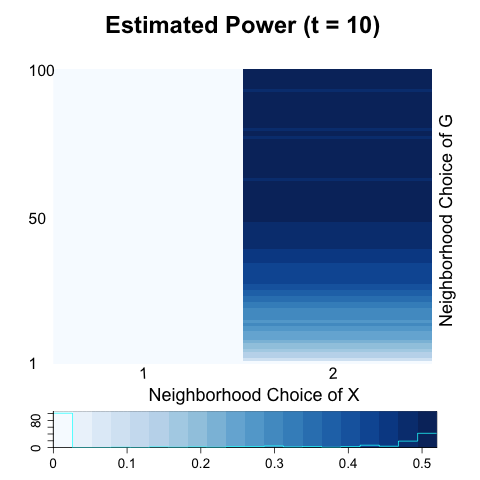
\includegraphics[width=2in]{../Figure/twoSBM_power10.png}
	\caption{Empirical power heatmap at diffusion time point $t=1$(left), $t=5$(middle), and $t=10$(right) based on $M = 500$ independently generated SBM presented in Eq.~\ref{eq:twoSBM}}
	\label{fig:twoSBM_power}
\end{figure}
\begin{figure}[H]
	\centering
	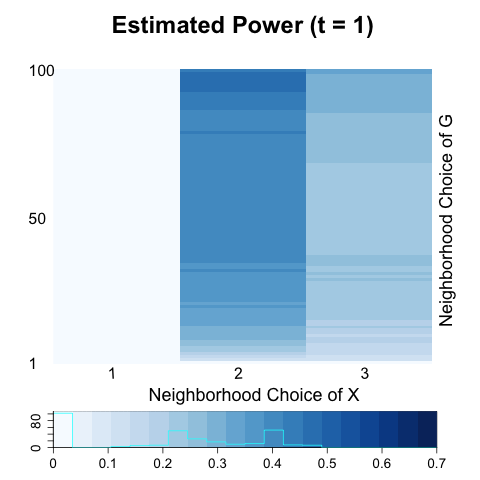
\includegraphics[width=2in]{../Figure/ThreeSBM_power1.png}
	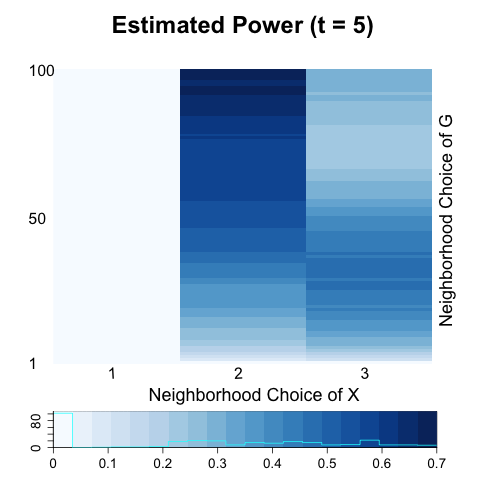
\includegraphics[width=2in]{../Figure/ThreeSBM_power5.png}
	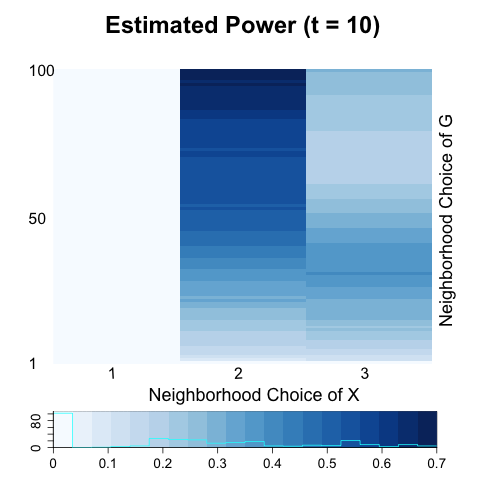
\includegraphics[width=2in]{../Figure/ThreeSBM_power10.png}
	\caption{Empirical power heatmap at diffusion time point $t=1$(left), $t=5$(middle), and $t=10$(right) based on $M = 500$ independently generated SBM presented in Eq.~\ref{eq:Three}}
	\label{fig:ThreeSBM_power}
\end{figure}


\begin{figure}[H]
	\centering
	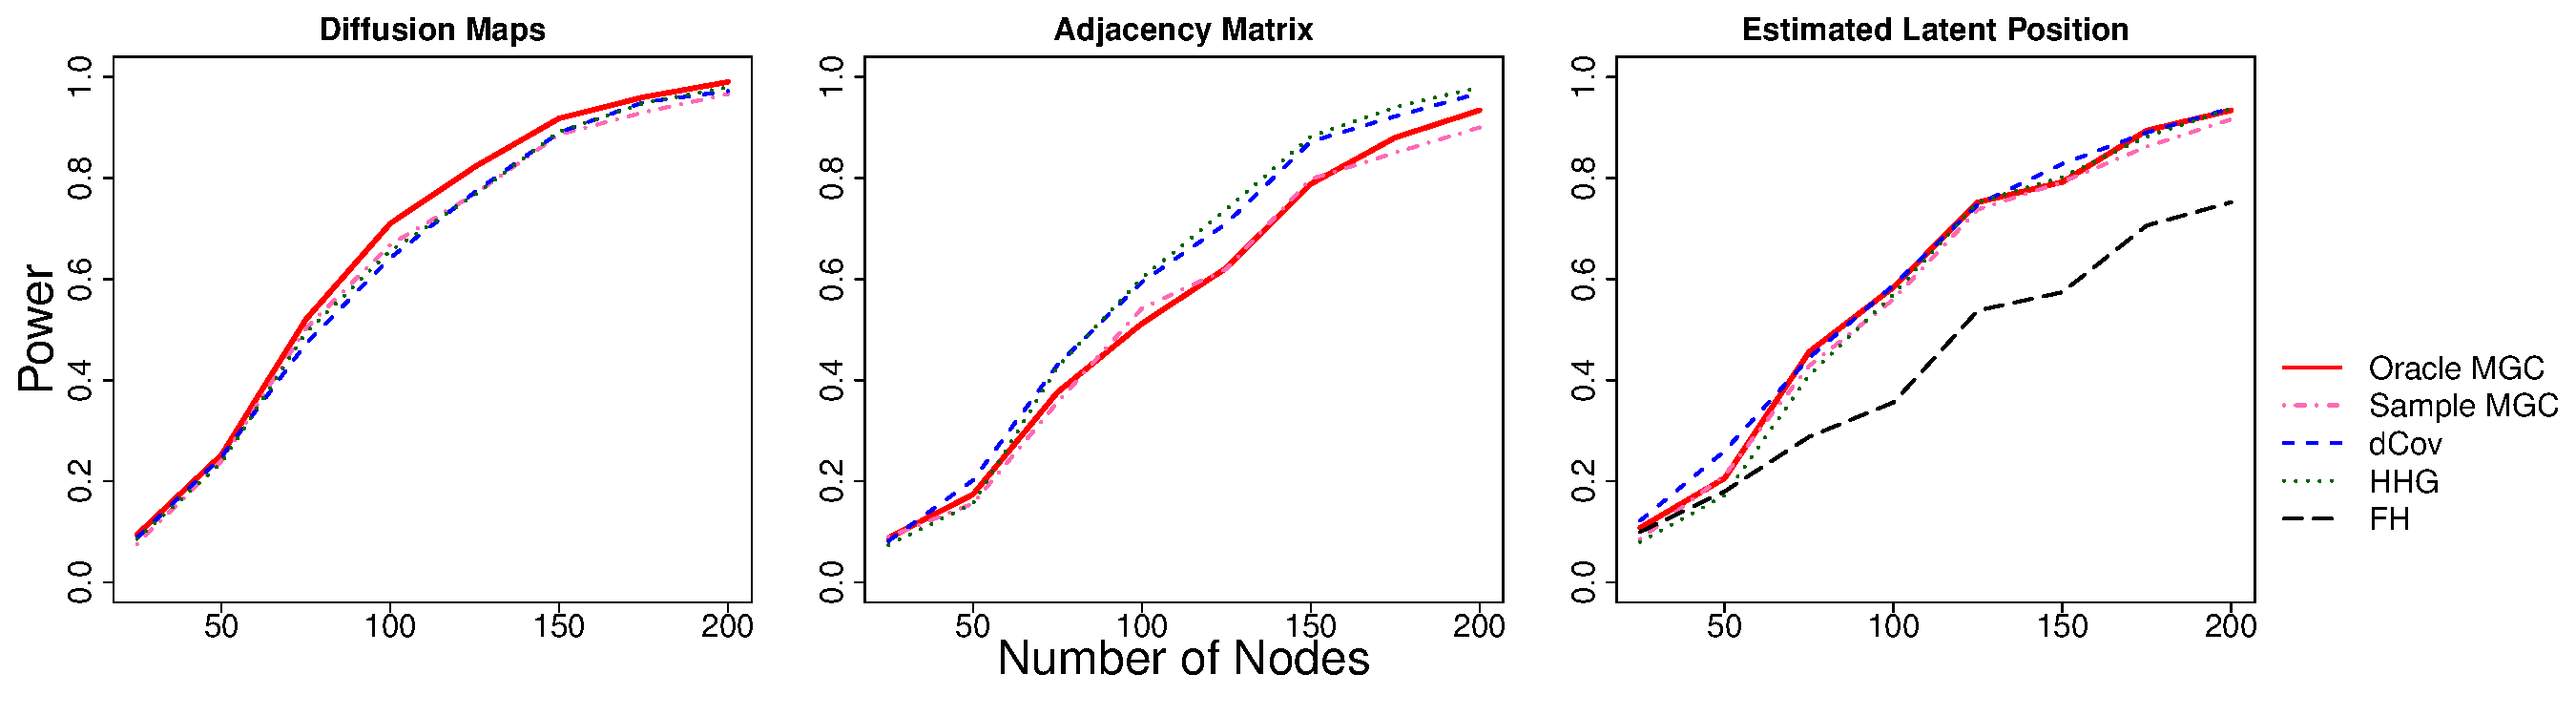
\includegraphics[width=7in]{../Figure/simplethreeSBM.pdf}
	\caption{Empirical power based on $M = 500$ of three SBM under linear dependence using diffusion maps (left), Euclidean of adjacency matrix (middle) and estimated latent position(right). The most right figure contains the results of \texttt{FH} test as well.}
	\label{fig:threeSBM}
\end{figure}


\subsection{exploratory analysis}



\textbf{Mixed Gaussian attributes and SBM}


\begin{figure}[H]
	\centering
	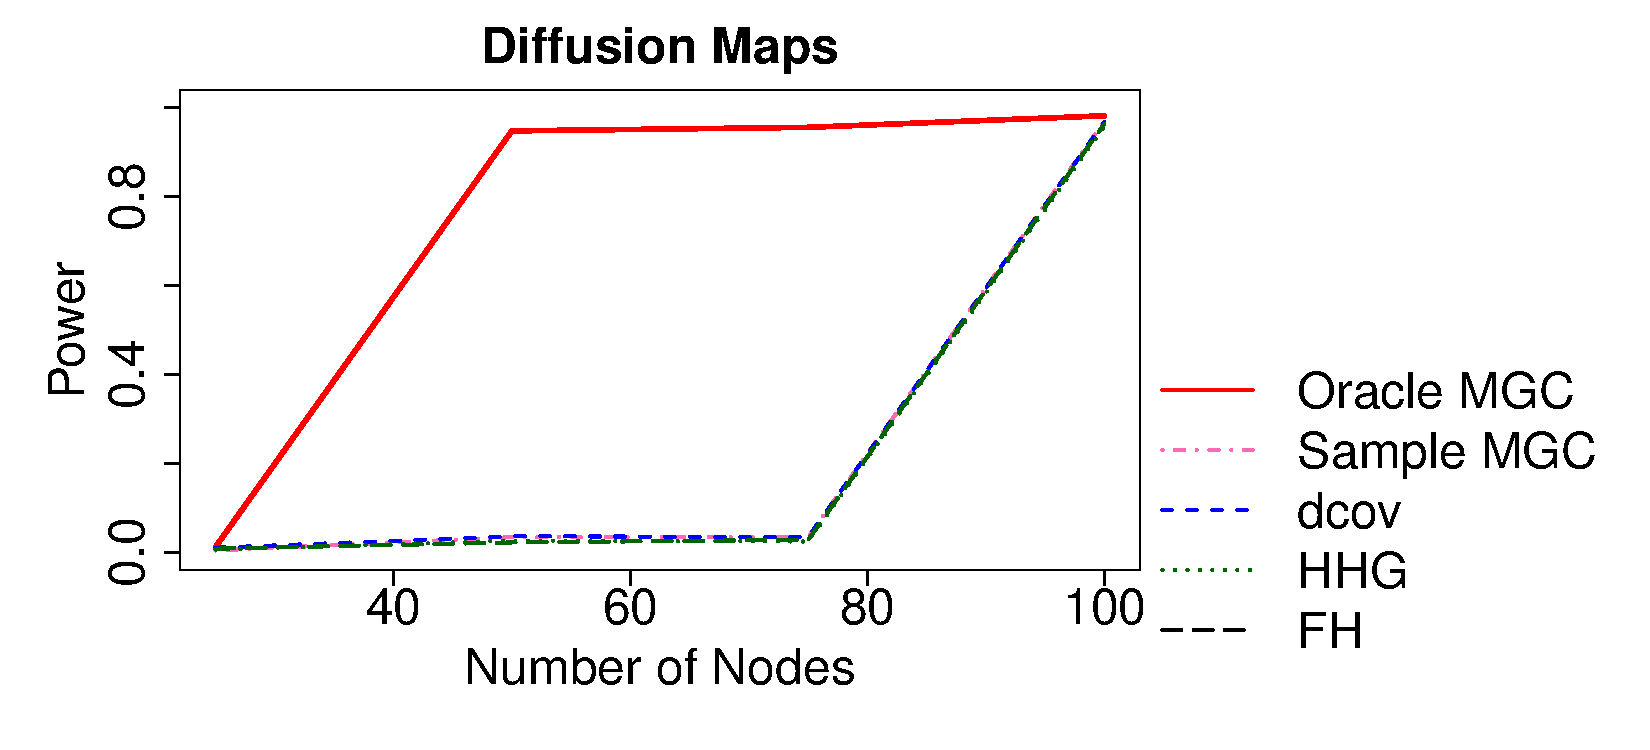
\includegraphics[width=5in]{../Figure/tmp_gaus.pdf}
	\caption{Empirical power based on $M = 500$ networks using diffusion maps.}
	\label{fig:threeSBM}
\end{figure}



\begin{figure}[H]
	\centering
	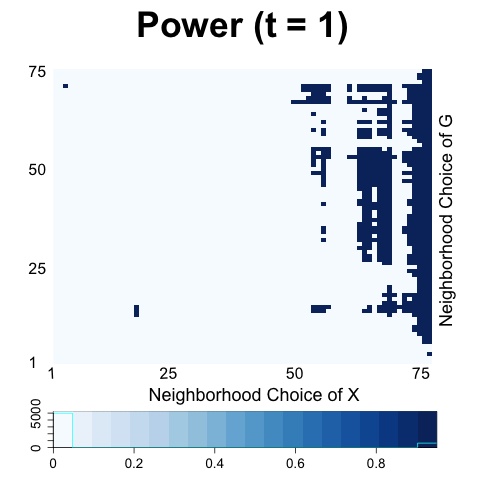
\includegraphics[width=2in]{../Figure/gaus_power1.png}
	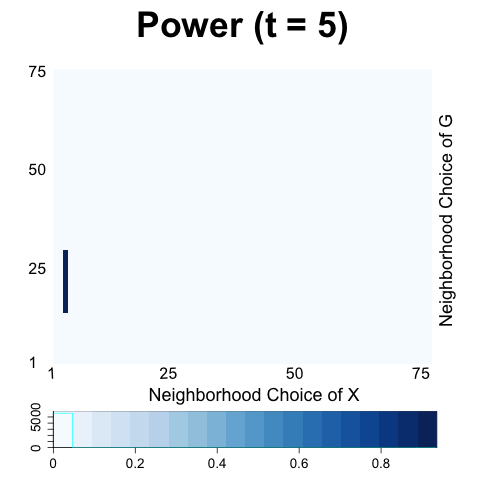
\includegraphics[width=2in]{../Figure/gaus_power5.png}
	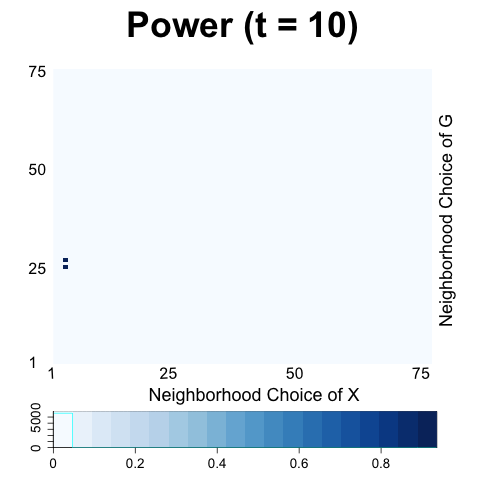
\includegraphics[width=2in]{../Figure/gaus_power10.png}
	\caption{Empirical power heatmap at diffusion time point $t=1$(left), $t=5$(middle), and $t=10$(right) based on $M = 500$ independently generated networks}
\end{figure}





%%%%%%%%
\textbf{Node Contribution}

\begin{figure}[H]
	\centering
	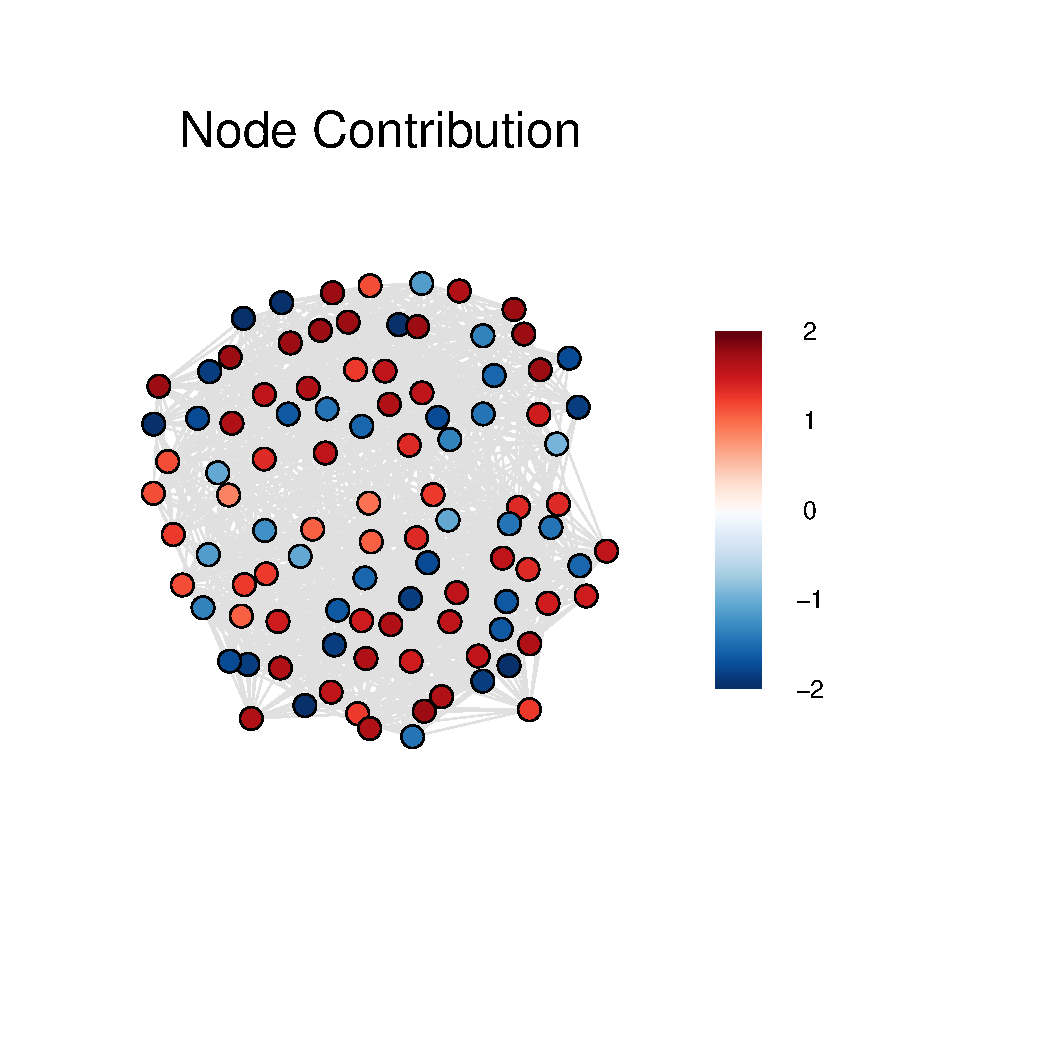
\includegraphics[width=2.3in]{../Figure/twoSBM_weight.pdf}
	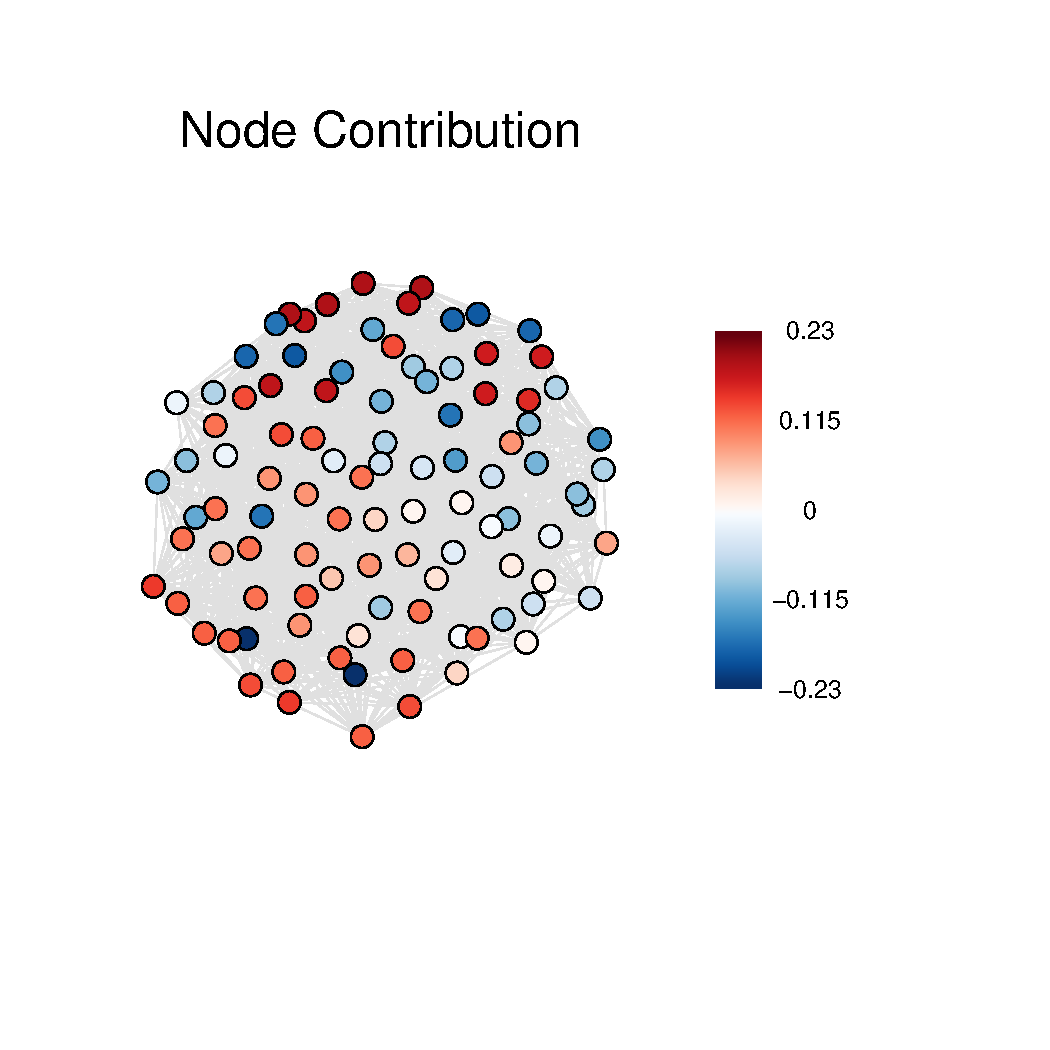
\includegraphics[width=2.3in]{../Figure/ThreeSBM_weight.pdf}
	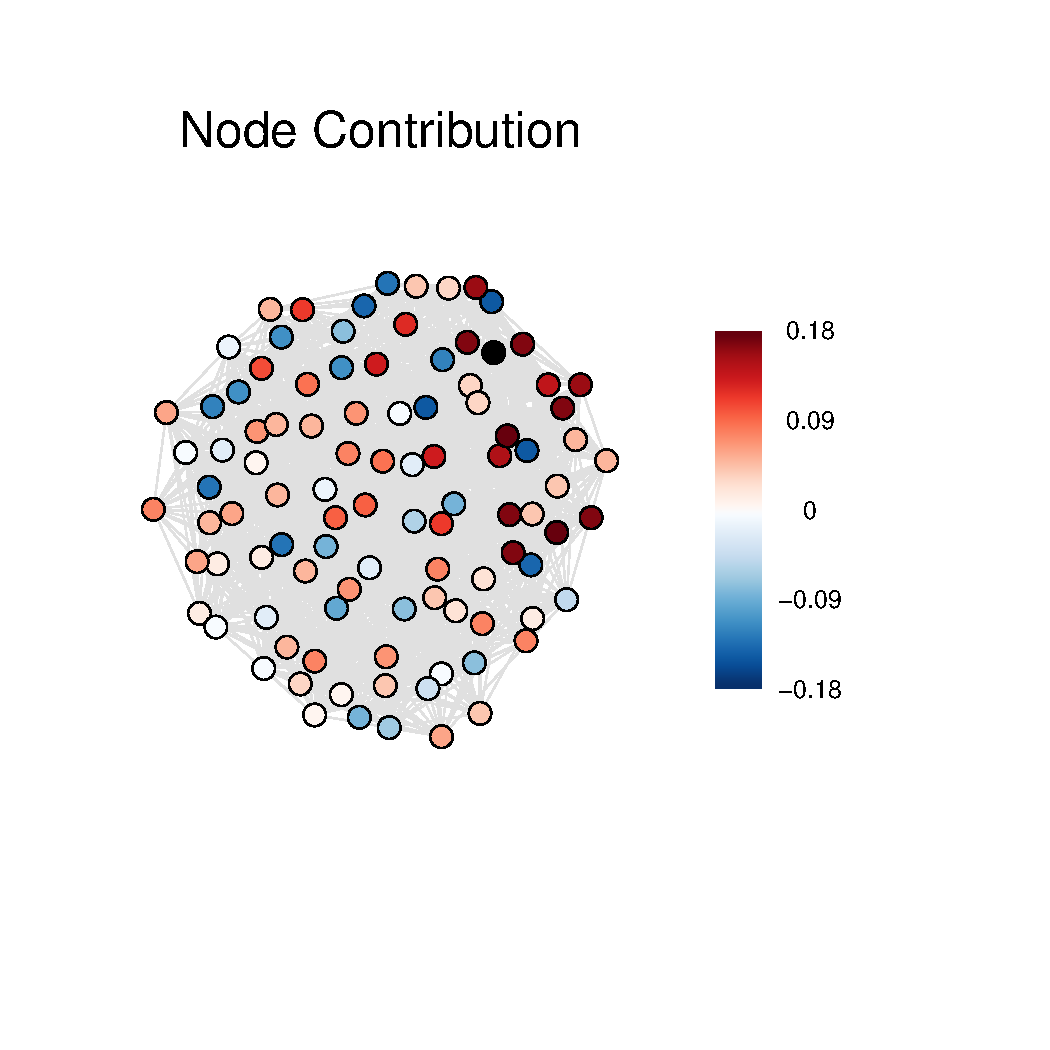
\includegraphics[width=2.3in]{../Figure/simplethree_weight.pdf}
	\caption{Node-specific contribution to testing independence in model~\ref{eq:twoSBM} (left), ~\ref{eq:Three} (middle) and ~\ref{eq:simplethree} (right).}
	\label{fig:weight1}
\end{figure}

\begin{figure}[H]
	\centering
	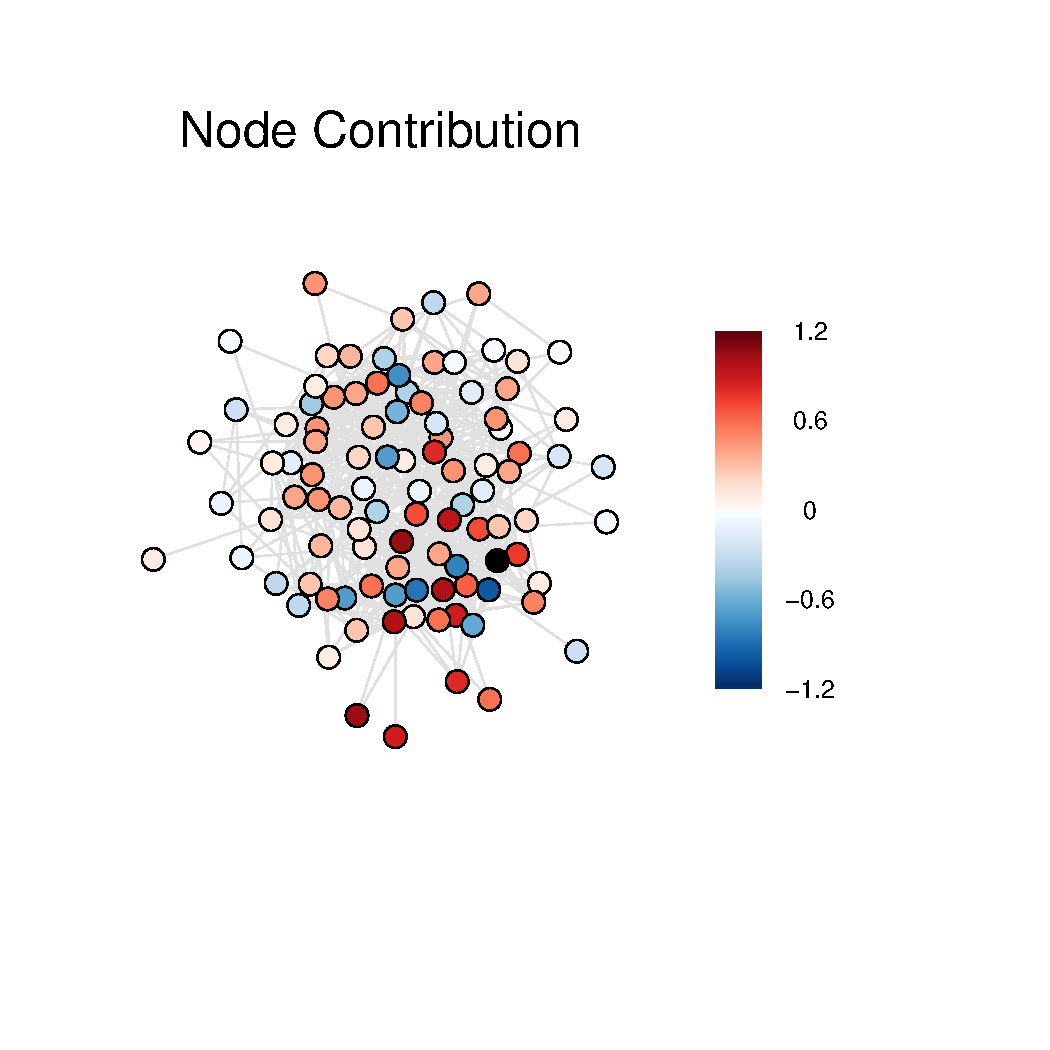
\includegraphics[width=3in]{../Figure/dcSBM_weight.pdf}
	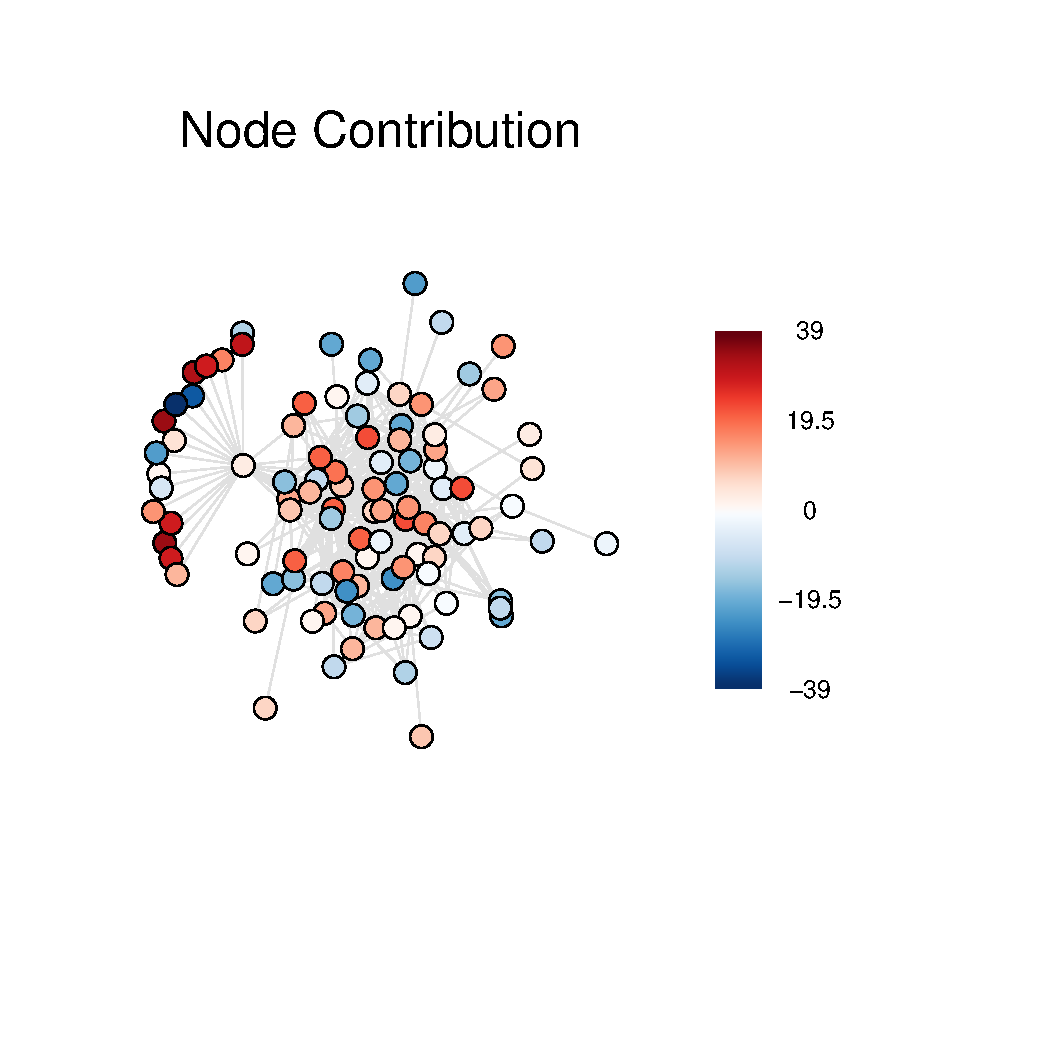
\includegraphics[width=3in]{../Figure/ame_weight.pdf}
	\caption{Node-specific contribution to testing independence in model~\ref{eq:dcSBM} (left) and ~\ref{eq:ame} (right).}
	\label{fig:weight2}
\end{figure}


%%%%%%%%%%%%%%%%%%%%%%%%%%%%%%%%%%%%%%%%%%%%%
\newpage
\subsection{Algorithms}
\alglanguage{pseudocode}

\begin{algorithm}[H]
	\caption{Mutiscale representation of nodes in network}
	\begin{algorithmic}[1]
		\Require Transition probability matrix of network $G$ and time points($\in N$) of diffusion time. 
		\Ensure A list of diffusion maps at each time point.
		\Function{ \texttt{dmap} }{ $n \times n$ transition matrix $P$, time points $\{ t_{1}, t_{2}, \ldots, t_{K} \}$ } 
		\State $\mathbf{\pi} :=$ \texttt{statdistr}($P$)\Comment{stationary distribution of $P$} 
		\State $\Pi : =$ \texttt{Diag}($\mathbf{\pi}$)\Comment{Diagonal matrix with diagonal element of $\mathbf{\pi}$}
		\State $Q: = \Pi^{1/2} P \Pi^{-1/2}$ 
		\State $\lambda := $ \texttt{eigenvalue}($Q$)\Comment{a real-valued vector with length of $q (\leq n)$. }
		\State $\Lambda : =$ \texttt{Diag}($\lambda$)
		\State $\Psi : =$ \texttt{eigenfunction}($Q$)\Comment{$n \times q$ real-valued matrix} 
		\State $\Phi :=  \Pi^{-1/2} \Psi$\Comment{$n \times q$ real-valued eigenfunction matrix of $P$}
		\For{$t_{i}$ :  $i$ = 1 }{ $K$}
		\Begin
		\State \texttt{Maps}$[i] := \Phi \Lambda^{t_{i}}$  
		\End
		\EndFor
		\State \texttt{Maps} = list( \texttt{Maps}[1], \texttt{Maps}[2], $\ldots$, \texttt{Maps}[$K$]  )
		
		\Return \texttt{Maps}
		\EndFunction
	\end{algorithmic}
\end{algorithm}

%%%%%%%%%%%%%%%%%%%%
\begin{algorithm}[H]
	\caption{Multiscale Generalized Correlation (\texttt{MGC}) test statistics when diffusion maps are applied.}
	\begin{algorithmic}[1]
		\Require A connected, undirected network $G$ with its nodal attributes $\mathbf{X}$.
		\Ensure A list of \big(  (a) p-value of \texttt{sample MGC}, (b) estimated \texttt{sample MGC} statistic, (c) p-value map for all local correlations, (d) a set of estimated optimal neighborhood scales $\{  (k^{*}, l^{*}  ) \}$  \big) for each diffusion maps.
		\Function{ \texttt{NetworkTest} }{ $G$, $\textbf{X}$,  $\mathbf{T}$ := (diffusion time points $\{ t_{1}, t_{2}, \ldots, t_{K} \}$)  }
		\State $A :=$ \texttt{get.adjacency}$(G)$\Comment{obtain an adjacency matrix of network $G$}
		\State $P := A $ / \texttt{rowSums}($A$) 
		\State $U :=$ \texttt{dmap}($P$, $\mathbf{T}$) \Comment{a list of diffusion maps in each time point}
		\For{$t_{i}$ :  $i$ = 1 }{ $K$}
		\Begin
		\State $C : =$  \texttt{dist}($U[i]$) \Comment{distance matrix of diffusion maps at time $t_{i}$}
		\State $D : =$ \texttt{dist}($X$) \Comment{distance matrix of nodal attributes}
		\State \texttt{MGC}$[i]$ = \texttt{MGCPermutationTest}( $C$, $D$ ) 
		\End
		\EndFor
		\State \texttt{MGC} = list( \texttt{MGC}[1], \texttt{MGC}[2], $\ldots$, \texttt{MGC}[$K$]  )
		
		\Return \texttt{MGC}
		\EndFunction
	\end{algorithmic}
\end{algorithm}



%%%%%%%%%%%%%%%%%%%%%%
\begin{algorithm}[H]
	\caption{Node-specific contribution to detecting dependency via \texttt{MGC} statistic}
	\begin{algorithmic}[1]
		\Require Distance metric of $G$ and $X$ for each and (one of) the estimated optimal scales $\{ k^{*}, l^{*} \}$ 
		\Ensure  Standardized contributions of each node in network $\{  c(v) \}$
		\Function{ \texttt{Contribution} }{   C, D , $\{  (k^{*}, l^{*}) \}$   }
		\State $\tilde{C} : = \texttt{DoubleCentering}(C)$
		\State $\tilde{D} := \texttt{DoubleCentering}(D)$
		\State \texttt{Rank}($M_{i}$):= (rank of node $i$'s nearest neighbors in terms of distance matrix $M$)
		\For{$v = 1$}{ $n$}
		\State $c(v) = 0$
		\For{$j = 1$}{ $n$}
		\Begin
		\State $c(v) =  c(v) + \tilde{C}_{vj} \tilde{D}_{v j} I(  \texttt{Rank}(C_{v})  \leq k^{*}, \texttt{Rank}(D_{v}) \leq l^{*} )$
		\State  $c(v) = c(v) + \tilde{C}_{jv} \tilde{D}_{jv} I(  \texttt{Rank}(C_{j}) \geq k^{*}, \texttt{Rank}(D_{j}) \leq l^{*} )$
		\End
		\EndFor
		\State $c(v) = c(v) / 2 n^2$
		\EndFor
		\State \texttt{cset} $:= \{ c(v) : v = 1,2, \ldots ,n  \}$
		
		\Return  \texttt{cset}
		\EndFunction
	\end{algorithmic}
\end{algorithm}

%%%%%%%%%%%%%%%%%%%%%%%%%%%%%%%%%%%%%%%%%%%%%	
\newpage
\subsection{Lemmas and Theorems}
	
\begin{theorem}[de Finetti's Theorem] 
	\label{finetti}
	
\bigskip			
1. Let $X_{1}, X_{2}, ...$ be an infinite sequence of random variables with values in a space $\mathbf{X}$. The sequence $X_{1}, X_{2}, ...$ is exchangeable \textit{if and only if} there is a random probability measure $\eta$ on $\mathbf{X}$ such that the $X_{i}$ are conditionally i.i.d. given $\eta$. 
		
2. If the sequence is exchangeable, the empirical distributions
		
$$\hat{S}_{n} ( . ) := \frac{1}{n} \sum\limits_{i=1}^{n} \delta_{X_{i}} ( .), n \in \mathbb{N}$$
		converges to $\eta$ as $n \rightarrow \infty$ with probability 1.
\end{theorem}
	
\begin{theorem}[Aldous Hoover Theorem]
		\label{Aldous_Hoover}
		
		Let $\mathbf{A} = \{A_{ij}\}, 1 \leq i,j \leq \infty$ be a jointly exchangeable binary array if and only if there exists a random measurable function $f : [0,1]^{3} \rightarrow \mathbf{A}$ such that 
		
		\begin{equation}
		\big(  A_{ij}  \big) \stackrel{d}{=} \left( f \big( U_{i}, U_{j}, U_{ij} \big)  \right)
		\end{equation}
		where $(U_{i})_{i \in \mathbb{N}}$ and $(U_{ij})_{i,j > i \in \mathbb{N}}$ with $U_{ij} = U_{ji}$ are a sequence and matrix, respectively, of i.i.d. Uniform[0,1] random variables. 
\end{theorem}
	
%%%%%%%%%%%%%%%%%%%%%%%%%%%%%%%%%%%%%%%%%%%%%%%%%		
\begin{proof}[\textbf{Proof of Lemma~\ref{lemma_graphon} }] 
	By \textit{Aldous-Hoover Theorem}~\ref{Aldous_Hoover}, a random array $(A_{ij})$ is jointly exchangeable \textit{if and only if} it can be represented as follows : 
		
	There is a random function $g : [0,1]^2 \rightarrow [0,1]$ such that 
\begin{equation}
(A_{ij})  \stackrel{d}{=} Bern( g(W_{i}, W_{j}))
\end{equation}
where $W_{i} \overset{i.i.d.}{\sim} Uniform(0,1)$. Thus if $\mathbf{A}$ is an adjacency matrix of an undirected, exchangeable network, for any $i < j,$ $i,j = 1,... , n$:
\begin{equation}
\begin{split}
	P \big(  A_{ij} = a_{ij} \big) & = \int P \big( A_{ij} \big| w_{i}, w_{j} \big) Pr(W_{i} = w_{i}) Pr(W_{j} = w_{j}) dw_{i} dw_{j} \\ & = \int_{0}^{1} \int_{0}^{1} g( w_{i},  w_{j})^{a_{ij}} \big( 1- g( w_{i},  w_{j}) \big)^{1-a_{ij}} dw_{i} dw_{j} 
\end{split}
\end{equation}
		
Then within each row, adjacent elements are independent and also identically distributed except a diagonal element.

\end{proof}
	

%%%%%%%%%%%%%%%%%%%%%%%%%%%%%%%%%%%%%%%%	
\begin{proof}[\textbf{Proof of Lemma~\ref{main_lemma}}]
We have shown that for fixed time $t$, diffusion distance is defined as an Euclidean distance of diffusion maps. Diffusion map is represented as follows :
\begin{equation}
	\mathbf{U}_{t}(i) = \begin{pmatrix} \lambda^{t}_{1} \phi_{1}(i) & \lambda^{t}_{2} \phi_{2} (i)  & \cdots & \lambda^{t}_{q} \phi_{q}(i) \end{pmatrix} \in \mathbb{R}^{q}.
\end{equation}
where $\Phi = \Pi^{-1/2}\Psi$ and $Q= \Psi \Lambda \Psi^{T} = \Pi^{1/2} P \Pi^{-1/2}$. 
Thus $P \Pi^{-1/2} \Psi = \Pi^{-1/2} \Psi \Lambda$. 
Then for any $r$th row ($r \in \{1,2, ... , q \}$, $(q \leq n)$), we can see that $P \phi_{r} = \lambda_{r} \phi_{r}$  where $\phi_{r} = \begin{pmatrix}  \psi_{r}(1) / \sqrt{\pi(1)} &  \psi_{r}(2) /  \sqrt{\pi(2)} & \cdots & \psi_{r}(n) /  \sqrt{\pi(n)}  \end{pmatrix}$.
Therefore to guarantee exchangeability (or \textit{i.i.d}) of $\mathbf{U}_{t}$, it suffices to show exchangeability (or \textit{i.i.d}) of $P$.

Assume joint exchangeability of $\mathbf{G}$, i.e. $(A_{ij}) \stackrel{d}{=} \big( A_{\sigma(i) \sigma(j)} \big)$. 
Since $A_{ij}$ is binary, $A_{ij} / \sum\limits_{ij} A_{ij} = A_{ij} /  (1 + \sum\limits_{l \neq j} A_{il})$. Moreover, $A_{ij}$ and $(1 + \sum\limits_{l \neq j} A_{il})$ are independent given its link function $g$, and $A_{\sigma(i) \sigma(j)}$ and $(1 + \sum\limits_{l \neq j} A_{\sigma(i) \sigma(l)})$ are independent also given $g$.
Then the following joint exchangeability of transition probability holds for $i \neq j; i,j = 1,2, \ldots,n$:

\begin{equation}
\big( P_{ij} \big) = \left(  \frac{A_{ij}}{1 - A_{ij} + \sum\limits_{j=1}^{n} A_{ij} } \right)  \stackrel{d}{=} \left( \frac{A_{\sigma(i) \sigma(j)} }{1 - A_{\sigma(i) \sigma(j)} + \sum\limits_{\sigma(j) = 1}^{n} A_{\sigma(i) \sigma(j)} } \right) = \big( P_{\sigma(i) \sigma(j)} \big)
\end{equation}
		
When $i = j$, $P_{ij} = P_{\sigma(i) \sigma(j)} = 0$ for $i=1,2, \ldots, n$.
Thus, transition probability is also exchangeable. 
This results exchangeable eigenfunctions $\{ \Phi(1), \Phi(2), , ... , \Phi(n) \}$ 
where $\Phi(i) := \begin{pmatrix} \phi_{1}(i) & \phi_{2}(i) & \cdots & \phi_{q}(i) \end{pmatrix}^{T}$, $i=1,2, \ldots, n$. Thus diffusion maps at fixed $t$, $\mathbf{U}_{t} = \begin{pmatrix} \Lambda^{t} \Phi(1)  & \Lambda^{t} \Phi(2) & \cdots & \Lambda^{t} \Phi(n)  \end{pmatrix}$ are exchangeable.  Furthermore by \textit{de Finetti's Theorem}~\ref{finetti}, we can say that $\mathbf{U}(t) = \{ U^{(t)}_{1}, U^{(t)}_{2}, ... , U^{(t)}_{n} \}$ are conditionally independent on a random probability measure $\eta$. 
\end{proof}
	
%%%%%%%%%%%%%%%%%%%%%%%%%%%%%%%%%%%%%%%%%%%	
\begin{proof}[\textbf{Proof of Lemma~\ref{lemma_graphex}}]
	Based on Kallenberg and Exchangeable Graph (KEG) frameworks, introduced in \cite{veitch2015class}, a random array $(A_{ij})$ is jointly exchangeable \textit{if and only if} it can be represented as follows : there is a random function $g : \mathbb{R}^{2}_{+} \rightarrow [0,1]$ such that 
	
	\begin{equation}
	(A_{ij})  \stackrel{d}{=} (A_{v_{i}, v_{j}} )  \stackrel{d}{=} Bern( g( \vartheta_{i}, \vartheta_{j}))
	\end{equation}
	where $v_{i} \overset{i.i.d.}{\sim} Poisson(1), \vartheta_{i} \overset{i.i.d.}{\sim} Poisson(1), v_{i} \leq \nu, i = 1,2,... , n$, for some pre-specified $\nu >0$ so that finite size graphs can include vertices only if they participate in at least one edges. Thus if $\mathbf{A}$ is an adjacency matrix of such undirected, exchangeable network, for any $i < j,$ $i,j = 1,... , n$:
\begin{equation}
\begin{split}
	P \big(  A_{ij} = a_{ij} \big| V_{i}, V_{j} \big) & = \int P \big( A_{ij} \big| v_{i}, v_{j} \big) Pr(\vartheta_{i} = \vartheta_{i}) Pr(\vartheta_{j} = \vartheta_{j})   dv_{i} dv_{j} d\vartheta_{i} d\vartheta_{j}   \\ & = \int_{0}^{\tau} \int_{0}^{\tau}   \int_{0}^{\infty} \int_{0}^{\infty}  g( \vartheta_{i},  \vartheta_{j})^{a_{ij}} \big( 1- g( \vartheta_{i},  \vartheta_{j}) \big)^{1-a_{ij}}  \\ & \quad \times dPois_{1}(\vartheta_{i}) \times dPoi_{1}(\vartheta_{j})  d \vartheta_{i} d \vartheta_{j}.
\end{split}
\end{equation}
\end{proof}
where $dPois_{1}(\cdot)$ is a probability distribution function of Poisson process with rate of 1.  Thus given $\{ \mathbf{V} \}$, edge probability except self-loop within each row (or column) is conditionally $\textit{i.i.d}$ given a link function $g$ and Poisson process $V$.

%%%%%%%%%%%%%%%%%%%%%%%%%%%%%%%%%%%%%%%%%%%%%%	
\begin{proof}[\textbf{Proof of corollary~\ref{corollary1}}][Triangle inequality of diffusion distance]
Let $x, y, z \in V(G).$
	
\begin{equation}
\begin{split}
D^{2}_{t}(x,z) & = \sum\limits_{w \in V(G)} \big( P^{t}(x,w) - P^{t}(z,w)   \big)^2 \frac{1}{\pi(w)}  \\ & = \sum\limits_{w \in V(G)} \big(P^{t}(x, w) - P^{t}(y,w) + P^{t}(y,w) - P^{t}(z,w) \big)^2 \frac{1}{\pi(w)} \\ & = \sum\limits_{w \in V(G)} \big( P^{t}(x,w) - P^{t}(y,w) \big)^2 \frac{1}{\pi(w)}  + \sum\limits_{w \in V(G)} \big( P^{t}(y,w) - P^{t}(z,w)  \big)^2 \frac{1}{\pi(w)} \\ & + 2 \sum\limits_{w \in V(G)} \big( P^{t}(x,w) - P^{t}(y,w)  \big) \big( P^{t}(y,w) - P^{t}(z,w)  \big)\frac{1}{\pi(w)} \\ &= D^{2}_{t}(x,y) + D^{2}_{t}(y,z) +  2 \sum\limits_{w \in V(G)} \big( P^{t}(x,w) - P^{t}(y,w)  \big) \big( P^{t}(y,w) - P^{t}(z,w)  \big)\frac{1}{\pi(w)}   
\end{split}
\end{equation}
	
Thus it suffices to show that 
	
\begin{equation}
\sum\limits_{w \in V(G)} \big( P^{t}(x,w) - P^{t}(y,w)  \big) \big( P^{t}(y,w) - P^{t}(z,w)  \big)\frac{1}{\pi(w)} \leq D_{t}(x,y) \cdot D_{t}(y,z). 
\end{equation}
	
Let $a_{w} = \big(P^{t}(x,w) - P^{t}(y,w) \big) \sqrt{1 / \pi(w)}$ and $b_{w} = \big( P^{t}(y,w) - P^{t}(z,w) \big) \sqrt{1 / \pi(w)}$. Then the above inequality is equivalent to :
	
\begin{equation} 
\sum\limits_{w \in V(G)} a_{w} \cdot b_{w} \leq \sqrt{\sum\limits_{w \in V(G)} a^2_{w} \cdot \sum\limits_{w \in V(G)} b^2_{w} }.
\end{equation}
which is true by Cauchy-Schwarz inequality.
\end{proof}	

%%%%%%%%%%%%%%%%%%%%%%%%%%%%%%%%%%%%%%%%%%%%%%%%
\begin{proof}[\textbf{Proof of Lemma~\ref{lemma1}} Convergence of empirical characteristic function of exchangeable variables] 
	
This follows exactly the same as \textit{Theorem 1} in \cite{szekely2007measuring}. Note that this lemma always holds without any assumption on $\{(\mathbf{x}_{j},\mathbf{y}_{j}), j=1,2,...,n\}$, e.g., it holds without assuming exchangeability, nor identically distributed, nor finite moments.
\end{proof}


\begin{proof}[\textbf{Proof of Lemma~\ref{lemma2}} Empirical characteristic function of exchangeable variables] 
\bigskip	
It suffices to prove the first argument~\ref{eq:conv1} since the second argument~\ref{eq:conv2} immediately follows from the first one by the property of characteristic functions.
Proving the first one is equivalent to \textit{Theorem 2} in \cite{szekely2007measuring}. However, they required $\{(\mathbf{x}_{i},\mathbf{y}_{i})\}$ to be independently identically distributed as $(\mathbf{x},\mathbf{y})$ with finite second moments; here we have exchangeable $\{ ( \mathbf{x}_{i}, \mathbf{y}_{i}  ) \}$ instead. 


Followied by \textit{de Finetti's Theorem}~\ref{finetti}, if and only if $\{ x_{i} \}$ are (infinitely) exchangeble, there exist an underlying distribution $f_{\mathbf{x}}$ of $\mathbf{x}$ such that $\mathbf{x}_{i}  \overset{i.i.d}{\sim} f_{\mathbf{x}} $. By the same logic there exists a random, we have an underlying distribution $f_{\mathbf{y}}$ where $\mathbf{y}_{i} \overset{i.i.d}{\sim} f_{\mathbf{y}}$. Let $(\mathbf{x}_{i}, \mathbf{y}_{i}) \overset{i.i.d}{\sim}   f_{\mathbf{x}, \mathbf{y}}$. Then under the assumption of finite second moment of the underlying distributions and measurable, conditioned random functions, we have a strong large number for V-statistics followed by \cite{szekely2007measuring}, i.e., 
\begin{eqnarray}
		\displaystyle\int_{D(\delta)}{\|g_{\mathbf{x},\mathbf{y}}^{n}(t,s)-g_{\mathbf{x}}^{n}(t)g_{\mathbf{y}}^{n}(s)\|^{2}}dw &\stackrel{n \rightarrow \infty}{\longrightarrow} 
		 \displaystyle\int_{D(\delta)}{\|g_{\mathbf{x},\mathbf{y}}(t,s)-g_{\mathbf{x}}(t)g_{\mathbf{y}}(s)\|^{2}}dw,
\label{eq:SLLN}
\end{eqnarray}
where $D(\delta)=\{(t,s):\delta \leq |t|_{p} \leq 1/\delta,\delta \leq |s|_{q} \leq 1/\delta\}$, and $w(t,s)$ is the weight function chosen in \cite{szekely2007measuring}. 
\end{proof}

%%%%%%%%%%%%%%%%%%%%%%%
\begin{proof}[\textbf{Proof of Theorem~\ref{theoremMain}} Consistency of \texttt{dCorr} applied to exchangeable variables]
\bigskip
Under the exchangeability and finite moments assumptions of underlying distribution, it follows from Lemma~\ref{lemma1} and ~\ref{lemma2} that $\mathcal{V}^{2}_{n}(\mathbf{X},\mathbf{Y}) \xrightarrow{n \rightarrow \infty}  0$ if and only if underlying distribution of $\{\mathbf{x}_{i} \}$, $\mathbf{x}$ is independent from underlying distribution of $\{ \mathbf{y}_{i}  \}$, $\mathbf{y}$. Therefore, the \texttt{dCorr} or \texttt{mCorr} converges to $0$ if and only if  underlying distributions are independent; and its testing power converges to $1$ under any joint distribution of finite moments. Since the multiscale generalized correlation based on any consistent global correlation is also consistent (see in [Cencheng]), \texttt{MGC} statistic constructed by \texttt{dCorr} or \texttt{mCorr} is also consistent in testing dependence.
\end{proof}

\begin{proof}[\textbf{Proof of Theorem~\ref{theorem2}} Consistency of \texttt{MGC} applied to exchangeable variables]

Suppose that we have undirected, connected network $\mathbf{G}$ with a family of diffusion maps $\{ \mathbf{u}_{t}  \}$ and with nodal attributes $\{ \mathbf{x}  \}$. We have shown in the Lemma~\ref{main_lemma} that $\{ \mathbf{u}_{t}  \}$ are exchangeable for each $t \in \mathbb{N}$. Thus there exists an underlying distribution of $\mathbf{u}_{t}$ such that $\mathbf{u} \overset{i.i.d}{\sim} f_{\mathbf{u}^{(t)}}$ for $t= 1,2,\ldots $; and we have $\mathbf{x}_{i} \overset{i.i.d}{\sim} f_{\mathbf{X}}$. Under the assumption of finite second moment of $\mathbf{u}^{(t)}$ and $\mathbf{x}$, \texttt{MGC} statistics constructed by $\{  (  \mathbf{u}_{ti}, \mathbf{x}_{i} ) : i = 1,2,\ldots, n  \}$ yield a consistent testing which determines the independence between underlying distributions of $\mathbf{u}^{(t)}$ and $\mathbf{x}$, followed by Lemma~\ref{lemma2}. 
From the same setting of network $\mathbf{G}$, we have estimated \textit{i.i.d} node-specific network factors $\{ \mathbf{F}_{i} \}$, we have n-pair of \textit{i.i.d} $\{ ( \mathbf{F}_{i}, \mathbf{x}_{i} )  \}$ and they can be applied it to \texttt{MGC} without assuming conditioning underlying distribution. In case of using adjacency matrix directly into test, we must assume the adjacency matrix comes from directed network $\mathbf{G}$, i.e. $A_{ij} \overset{i.i.d}{\sim} f_{A}$ for all $i,j=1,2,\ldots, n$; otherwise, each column is dependent on one another.  
\end{proof}


\bibliographystyle{Chicago}
\bibliography{Biblio}
	
%%%%%%%%%%%%%%%%%%%%%%%%%%%%%%%%%%%%%%%%%%	
\newpage
\bigskip
\begin{center}
	{\large\bf SUPPLEMENTARY MATERIAL}
\end{center}
	
All of the \texttt{R} functions and simulation data in \texttt{RData} format are provided in \url{https://github.com/neurodata/Multiscale-Network-Test}.
	
	
\end{document}